\chapter{A função \texorpdfstring{$\zeta$}{zeta} de Riemann}
\chaptermark{}

\hfill%
\begin{minipage}{10cm}
    \begin{flushright}
    \rightskip=0.5cm
        \textit{%
            ``If I were to awaken after having slept for a thousand years, my first question would be: Has the Riemann hypothesis been proven?''
        }
        \\[0.1cm]
    \rightskip=0.5cm
    --- David Hilbert
    \end{flushright}
\end{minipage}

\section{Funções Inteiras}
    \subsection{Fórmula de Jensen e número de zeros}
    
    Nesta seção, mostraremos o Teorema da Fórmula de Jensen, que relaciona os zeros 
    de uma função em um disco com a média logarítmica do módulo desta função ao 
    longo do bordo do disco. Não é claro, a princípio, o significado desta fórmula,
    mas ela permitirá que cheguemos a várias conclusões muito interessantes. 
    Vamos poder, por exemplo, estabelecer estimativas a respeito da quantidade 
    de zeros de uma função no interior de um disco de raio dado.
    
    Inicialmente, começamos mostrando dois resultados que nos serão bastante úteis.
    Primeiro, observe que, se $f$ é holomorfa num disco de raio $R$ e centro $z_0$,
    pela fórmula integral de Cauchy, com $\gamma = z_0 + re^{i\theta}$ e $0 < r < R$,
    temos
    %
    \begin{align*}
        f(z_0) &= \frac{1}{2\pi i}\int_\gamma \frac{f(w)}{w - z_0} \, dw \\
        &= \frac{1}{2\pi i} \int_{0}^{2\pi} \frac{f(z_0 + re^{i\theta})}{z_0 + re^{i\theta} - z_0} rie^{i\theta} \, d\theta \\
        &= \frac{1}{2\pi}\int_{0}^{2\pi}f(z_0 + re^{i\theta}) \, d\theta.
    \end{align*}
    %
    Portanto,
    %
    \begin{equation}
    \label{eq-representacao-int-re-f(z)}
        \Re(f(z_0)) 
        = \frac{1}{2\pi}\int_{0}^{2\pi}\Re(f(z_0 + re^{i\theta})) \, d\theta.
    \end{equation}
    %
    Anteriormente, tentamos definir um ramo para o logaritmo de uma função $f(z)$, 
    mas o princípio do argumento nos foi um obstáculo porque $f$ tinha um zero 
    no interior da região delimitada por $\y$. Tanto zeros quanto singularidades 
    podem trazer problemas  se quisermos fazer uma construção daquele tipo, justamente
    por conta do princípio do argumento. 
    
    Se $G$ é uma conjunto aberto simplesmente conexo contendo 1 e que não contém 0,
    podemos definir um ramo do logaritmo $F(z) = \log_G(z)$ tal que $F$ é holomorfa 
    em $G$ e coincide com o logaritmos de base $e$ num intervalo real contendo 1. 
    Além disso, $\exp(F(z)) = z$ para todo $z \in G$. Lembre-se que podemos definir
    %
    \begin{equation*}
        \ln{x} = \int_{0}^{x}\frac{1}{t} \, dt.
    \end{equation*}    
    %
    Tomando esta situação como inspiração, definimos
    %
    \begin{equation*}
        F(z) = \int_\y \frac{1}{z} \, dz,
    \end{equation*}
    %
    onde $\y$ é uma curva contida em $G$ conectando 1 a $z$. Observe que $F$ está 
    bem definida, pois $G$ é um conjunto simplesmente conexo, ou seja qualquer 
    curva fechada é homotópica a zero, como no Teorema de Monodromia 
    (Teorema \ref{teo-monodromia}). Mais precisamente, se $\beta$ e $\y$ são 
    duas curvas contidas em $G$ conectando 1 a $z$, temos
    %
    \begin{equation*}
        \int_{\y * \beta^-} \frac{1}{z} \, dz = 0,
    \end{equation*}    
    %
    pois $1/z$ é holomorfa na região interior à concatenação dessas curvas. 
    A hipótese de $G$ ser simplesmente conexo é importante, pois, 
    num certo sentido, estamos fazendo continuações analíticas 
    no sentido do Teorema de Monodromia.
    
    Observe que 
    %
    \begin{equation*}
        \frac{d}{dz}F(z) = \frac{1}{z},
    \end{equation*}    
    %
    então 
    \begin{align*}
        \frac{d}{dz}(z\exp{-F(z)}) &= \exp{(-F(z))} + z\exp{(-F(z))}\frac{-1}{z} \\
        & = 0.
    \end{align*}
    %
    Como $G$ é conexo, concluímos que $z\exp{-F(z)}$ é constante. Calculando o 
    valor da expressão em $z = 1$, obtemos o resultado. Mostramos agora a última
    parte. Como $1 \in G$ e $G$ é aberto, existe um intervalo aberto 
    $I \subseteq \R$ contendo $1$ tal que, para $x \in I$,
    %
    \begin{equation*}
        F(x) = \int_{1}^{x} \frac{1}{t} \, dt = \ln{x}.
    \end{equation*}    
    %
    O próximo lema é, essencialmente, uma repetição dos argumentos acima, mas 
    num contexto mais geral.
    %
    \begin{lema}%Teorema 6.2 cap 3 Stein
    \label{lema-ramo-log}
        Se $f : G \to \C$ é holomorfa e não se anula na região simplesmente conexa 
        $G \subseteq C$, então existe uma função $g$ definida e holomorfa em $G$ 
        tal que 
        %
        \begin{equation*}
            f(z) = \exp{g(z)}
        \end{equation*}
        %
        para todo $z \in G$.
    \end{lema}
    %
    \begin{proof}
        Em termos práticos, $g(z) = \log f(z)$ se pudermos dar sentido a essa
        expressão. Seja $z_0 \in G$. Seguindo as ideias que mostramos anteriormente,
        definimos
        %
        \begin{equation*}
            g(z) = \int_{\y} \frac{f'(z)}{f(z)} \, dz, + C_0
        \end{equation*}
        %
        onde $\y$ é uma curva conectando $z_0$ a $z$ contida em $G$. Como $G$ é
        simplesmente conexo, $g$ está bem definida (i.e., independe da escolha de
        $\y$). A constante $C_0$ é escolhida de modo que $\exp(C_0) = f(z_0)$. 
        Além disso, observe que 
        %
        \begin{equation*}
            g'(z) = \frac{f'(z)}{f(z)}.
        \end{equation*}
        %
        Derivando a expressão $f(z)\exp{-g(z)}$ e usando a conexidade de $G$, vemos
        que ela é constante. O seu valor em $z = z_0$ é 1, então concluímos que 
        $f(z) = \exp{g(z)}$.
    \end{proof}
    %
    
    \medskip 
    
    
    A seguir, enunciamos e provamos o teorema que é o foco desta seção. O lema
    anterior e a observação no início da seção são usados fortemente para resolver
    integrais que seriam complicadas se tentássemos resolver explicitamente. 
    Denotamos por $D_R$ um disco centrado na origem com raio $R$.
    %
    \begin{teorema}[Fórmula de Jensen]
    \label{teo:form-jensen}
    \index{Fórmula!de Jensen}
    \index{Teorema!de Jensen}
        Sejam $G$ um aberto que contém o fecho do disco $D_R$ e $f$ uma função
        holomorfa em $G$ tal que $f(0) \neq 0$ e $f(z) \neq 0$ para 
        $z \in \partial D_R$. Denote por $z_1, \dots, z_N$ os zeros de $f$ no 
        interior de $D_R$ (listados com multiplicidade). 
        Então
        %
        \begin{equation}
        \label{eq-formula-jensen}
            \ln{|f(0)|} = \sum_{k = 1}^{N}\ln{\frac{|z_k|}{R}} 
            + \frac{1}{2\pi}\int_{0}^{2\pi}\ln{|f(Re^{i\theta})|} \, d\theta.
        \end{equation}
        %
    \end{teorema}
    %
    \begin{proof}
        Pelas propriedades do logaritmo e pela linearidade da integral, vemos que, 
        se duas funções satisfazem as hipóteses desse teorema, então o produto delas
        também satisfaz. Como os $z_j$ são os únicos zeros de $f$ no interior de
        $D_R$, a função $g:G -\{z_1, \dots, z_N\}\to \mathbb{C}$ dada por
        %
        \begin{equation*}
            g(z) = \frac{f(z)}{(z-z_1) \cdots (z-z_N)}
        \end{equation*}
        %
        tem apenas singularidades removíveis em $\overline{D}_R$. 
        Portanto podemos aplicar o Teorema de Riemann para
        garantir que $g$ admite uma extensão holomorfa, a todo $G$.  
        Além do mais, $g$ não se nula em $\overline{D}_R$. 
        Portanto temos
        %
        \begin{equation*}
            f(z) = (z-z_1)\cdots(z-z_N)g(z).
        \end{equation*}
        %
        Observe que se mostramos a validade da identidade
        \eqref{eq-formula-jensen} para funções do tipo $g(z)$ 
        (holomorfas e não se anulam em $\overline{D}_R$) e para as funções $z-z_j$ 
        o teorema fica demonstrado para $f$, pois ela é um produto destas funções.
        
        Como $G$ é aberto e contém $\overline{D}_R$, podemos encontrar $\Tilde{R}>R$
        tal que $D_{\Tilde{R}}$ está contido em $G$. Podemos, então, aplicar o 
        Lema \ref{lema-ramo-log} para a função $g$ e deduzir que existe uma função
        $h$ holomorfa em $D_{\Tilde{R}}$ tal que $g(z) = \exp(h(z))$. Segue que
        %
        \begin{equation*}
            |g(z)| = |\exp(h(z))| = e^{\Re{(h(z))}} 
            \implies \ln{|g(z)|} = \Re{(h(z))}.
        \end{equation*}
        %
        Usando última identidade acima e \eqref{eq-representacao-int-re-f(z)}
        a $\Re{(h(0))}$, obtemos 
        %
        \begin{align*}
            \ln{|g(0)|} = \Re(h(0)) &= \frac{1}{2\pi} 
            \int_{0}^{2\pi}\Re{(h(Re^{i\theta}))} \, d\theta \\
            &= \frac{1}{2\pi}\int_{0}^{2\pi}\ln{|g(Re^{i\theta})|} \, d\theta.
        \end{align*}
        %
        Mostrando a validade da Fórmula de Jensen para
        funções que não se anulam em $\overline{D}_R$.
        
        
        Resta mostrar que o resultado vale para uma função da forma $f(z) = z - w$,
        onde $w \in D_R$. Nosso objetivo é mostrar que vale
        %
        \begin{equation*}
            \ln{|w|} = \ln{\frac{|w|}{R}} 
            + \frac{1}{2\pi}\int_{0}^{2\pi}\ln{|Re^{i\theta} - w|} \, d\theta.
        \end{equation*}
        %
        Desenvolvendo os termos dessa soma onde é possível e notando que
        $|Re^{i\theta} - w| = R|e^{i\theta} - w/R|$, temos que o problema se 
        reduz a mostrar que vale
        %
        \begin{equation*}
            \int_{0}^{2\pi}\ln{|e^{i\theta} - a|} \, d\theta = 0,
        \end{equation*}
        %
        onde $|w/R| = |a| < 1$. Observe ainda que 
        $|e^{i\theta} - a| = |e^{i\theta}||1-ae^{i\theta}| = |1-ae^{i\theta}|$, 
        então reescrevemos a integral de interesse como
        %
        \begin{equation*}
            \int_{0}^{2\pi}\ln{|1 - ae^{i\theta}|} \, d\theta = 0.
        \end{equation*}
        %
        Explicitamente, esta integral se escreve como
        %
        \begin{equation*}
            \int_{0}^{2\pi}\ln{\sqrt{1 + |a|^2 - 2|a|\cos{\theta}}} \, d\theta,
        \end{equation*}
        %
        que não é tão simples de ser resolvida. A aplicação do 
        Lema \ref{lema-ramo-log} simplificará consideravelmente este cálculo. 
        
        Considere a função $F(z) = 1 - az$. $F$ não se anula e é holomorfa no 
        disco de raio $1$ centrado na origem, pois $|a| < 1$. Portanto, ela é
        holomorfa e não se anula num disco $D$ de raio $1 + \e$ centrado na origem,
        para algum $\e > 0$ suficientemente pequeno. 
        Este disco é uma região simplesmente
        conexa, então, pelo Lema \ref{lema-ramo-log}, existe uma função $G$ holomorfa
        em $D$ tal que 
        %
        \begin{equation*}
            F(z) = \exp(G(z)) \ \ \forall z \in D.
        \end{equation*}
        %
        
        Observe que $F(0) = 1$. Usando novamente a identidade
        \eqref{eq-representacao-int-re-f(z)} , temos
        %
        \begin{align*}
             0 = \ln{|F(0)|} &= \Re{(G(0))}\\
                &= \frac{1}{2\pi} \int_{0}^{2\pi}\Re{(G(e^{i\theta}))} \, d\theta \\
                &= \frac{1}{2\pi} \int_{0}^{2\pi}\ln{|F(e^{i\theta})|} \, d\theta \\
                &= \frac{1}{2\pi} \int_{0}^{2\pi}\ln{|1 - ae^{i\theta}|} \, d\theta .
        \end{align*}
        %
        O que encerra a prova do Teorema.
    \end{proof}
    
    
    
    
    \bigskip 
    
    
    
    Podemos ainda dar uma demonstração alternativa deste teorema que deixa mais explicita as ideias de extensão analítica contidas nesta demonstração. Observe que a fórmula de Jensen pode ser escrita na forma alternativa
    %
    \begin{equation*}
        \ln{\Big |f(0) \frac{R}{z_1}\cdots\frac{R}{z_N}\Big |} 
        = \frac{1}{2\pi}\int_{0}^{2\pi}\ln{|f(Re^{i\theta})|} \, d\theta, 
    \end{equation*}
    %
    onde usamos apenas as propriedades do logaritmo para reescrevê-la.
    
    Para uma função do tipo $g(z)$ acima, o teorema vale. Seja $f$ uma função
    satisfazendo as hipóteses do Teorema e considere a função
    %
    \begin{equation}\label{eq-aux-F-formula-jensen}
        F(z) = f(z)\frac{R^2 - z\overline{z}_1}{R(z-z_1)}\cdots
        \frac{R^2 - z\overline{z}_N}{R(z-z_N)}
    \end{equation}
    %
    definida em todo o $G$ exceto nos zeros de $f$. 
    Usando o Teorema de Riemann podemos garantir que $F$ admite uma extensão
    holomorfa a todo domínio $G$, 
    já que suas singularidades são todas removíveis. 
    Portanto, a menos de extensão, podemos assumir 
    que $F$ é uma função holomorfa em $G$. 
    Além disso, se $|z| = R$, então 
    %
    \begin{align*}
        \Big | \frac{R^2 - z\overline{z}_1}{R(z-z_j)} \Big | &= \Big | 
        \frac{R^2 - z\overline{z}_j}{R(z-z_j) \frac{R}{\overline{z}}} \Big | \\
        &= \Big | \frac{R^2 - z\overline{z}_j}{R^2-z_j\overline{z}}  \Big | \\
        &= 1.
    \end{align*}
    %
    Isto mostra que $|F(z)| = |f(z)|$ para todo $z \in \partial D_R$.
    Por hipótese, $f$ não anula $\partial D_R$. Consequentemente $F$ 
    não se anula no bordo de $D_R$. 
    Logo vale a fórmula de Jensen para $F$ e portanto
    %
    \begin{equation*}
        \ln{|F(0)|} = \frac{1}{2\pi}\int_{0}^{2\pi}\ln{|F(Re^{i\theta})|}\, d\theta.
    \end{equation*}
    %
    Usando a expressão de $F$ dada em 
    \eqref{eq-aux-F-formula-jensen}, 
    obtemos o resultado desejado.
    
    
    
    \bigskip 
    
    
    Agora, vamos usar a fórmula de Jensen para encontrar uma relação entre a
    taxa de crescimento de uma função inteira no infinito e o comportamento
    assintótico do número de zeros (contados com multiplicidade) desta
    função dentro dos discos $D(0,R)$ quando $R\to +\infty$.
    
    % Primeiro, note que podemos reescrever a fórmula de Jensen da seguinte forma:
    % %
    % \begin{align*}
    %     \ln|f(0)| = \sum_{j=1}^n \ln\left|\frac{z_j}{R}\right| 
    %     + \frac{1}{2\pi}\int_0^{2\pi} \ln|f(Re^{i\theta})| \, d\theta,
    % \end{align*}
    % %
    % usando as propriedades do logaritmo e do valor absoluto.
    
    Seja $f:U\subset\C\to\C$ é uma função holomorfa em $\overline{D(0,R)}$.
    Para cada $r\in (0,R)$ denotamos por $n_f(r) \equiv n(r)$ o número de zeros 
    de $f$, contados com multiplicidade, dentro do disco aberto $D(0,r)$.
    Note que segue diretamente da definição que se $0 < r_1 \leq r_2 < R$, então
    $n_f(r_1) \leq n_f(r_2)$, ou seja, $n_f$ é uma função não-decrescente. Usaremos
    esse fato no seguinte lema que, por sua vez, será o primeiro de dois resultados
    que nos permitirão extrair a relação entre: zeros e a ordem de uma função.
    
    % Vamos denotar por $n_f(r)$ o número zeros da função $f$ 
    % (contados com multiplicidade) no interior de um disco de raio $r$ e 
    % centro na origem. 
    % É fácil ver que $n_f$ é uma função não decrescente de $r$.
    %
    \begin{corolario}
    \label{corol:num-zeros}
        Se $z_1, \dots, z_N$ são os zeros de $f$ no interior de $D_R$, então
        %
        \begin{equation*}
            \int_{0}^{R}n_f(r) \, \frac{dr}{r} 
            = \sum_{k=1}^{N} \ln{\left |\frac{R}{z_k}\right|}.
        \end{equation*}
        %
    \end{corolario}
    %
    \begin{proof}
    Observe inicialmente que 
    %
    \begin{equation*}
        \ln{\left |\frac{R}{z_k}\right|} = \ln{R} - \ln{|z_k|} 
        = \int_{|z_K|}^{R} \, \frac{dr}{r}.
    \end{equation*}
    %
    Portanto, 
    %
    \begin{equation*}
        \sum_{k=1}^{N}\ln{\left |\frac{R}{z_k}\right|} 
        = \sum_{k=1}^{N}\int_{|z_k|}^{R} \, \frac{dr}{r}.
    \end{equation*}
    %
    Defina, para $k \in \{1, \dots, N\}$, as funções
    
    \begin{tabular}{%
    		@{}
    		m{.5\textwidth}
    		@{}
    		m{.5\textwidth}
    		@{}
    	}
    	\centering
    	$\dis
    	\eta_k(r) = 
        \begin{cases}
            1, &\text{se } r > |z_k| \\
            0, &\text{se } r \leq |z_k|
        \end{cases}
    	$
    	&
    	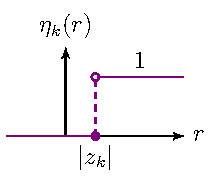
\includegraphics{Figuras/função salto.pdf} 
    \end{tabular}
    
    Então $n_f(r) = \dis{\sum_{k=1}^{N} \eta_k(r)}$. Segue que
    %
    \begin{align*}
        \sum_{k=1}^{N}\int_{|z_K|}^{R} \, \frac{dr}{r} 
        &= \sum_{k=1}^{N}\int_{|z_K|}^{R}\eta_k(r) \, \frac{dr}{r} \\
        &= \int_{|z_K|}^{R}\left(\sum_{k=1}^{N}\eta_k(r)\right) \, \frac{dr}{r} \\
        &= \int_{0}^{R}n_f(r) \, \frac{dr}{r}.
    \end{align*}
    %
    \end{proof}
    %
%\subsection{Ordem de crescimento e o número de zeros de uma função}
    % Agora, vamos usar a fórmula de Jensen para encontrar uma relação entre a
    % taxa de crescimento de uma função inteira no infinito e o comportamento
    % assintótico do número de zeros (contados com multiplicidade) desta
    % função dentro dos discos $D(0,R)$ quando $R\to +\infty$.
    
    % Primeiro, note que podemos reescrever a fórmula de Jensen da seguinte forma:
    % %
    % \begin{align*}
    %     \ln|f(0)| = \sum_{j=1}^n \ln\left|\frac{z_j}{R}\right| 
    %     + \frac{1}{2\pi}\int_0^{2\pi} \ln|f(Re^{i\theta})| \, d\theta,
    % \end{align*}
    % %
    % usando as propriedades do logaritmo e do valor absoluto.
    
    % Seja $f:U\subset\C\to\C$ é uma função holomorfa em $\overline{D(0,R)}$.
    % Para cada $r\in (0,R)$ denotamos por $n_f(r) \equiv n(r)$ o número de zeros 
    % de $f$, contados com multiplicidade, dentro do disco aberto $D(0,r)$.
    % Note que segue diretamente da definição que se $0 < r_1 \leq r_2 < R$, então
    % $n_f(r_1) \leq n_f(r_2)$, ou seja, $n_f$ é uma função não-decrescente. Usaremos
    % esse fato no seguinte lema que, por sua vez, será o primeiro de dois resultados
    % que nos permitirão extrair a relação entre zeros e a ordem de uma função.
    %
    % \begin{lema}
    % \label{lema:int-num-zeros}
    %     Sejam $R > 0$, $U\subseteq\C$ tal que $\overline{D(0,R)} \subseteq U$
    %     e $f:U\to\C$ uma função holomorfa. Se $z_1, z_2, \dots, z_n$ são zeros
    %     de $f$ em $D(0,R)$, então
    %     %
    %     \begin{equation*}
    %         \int_0^R n_f(r) \, \frac{dr}{r} 
    %         = \sum_{j=1}^n \ln\left|\frac{R}{z_j}\right|.
    %     \end{equation*}
    %     %
    % \end{lema}
    % %
    % \begin{proof}
    %     Note, primeiramente, que
    %     %
    %     \begin{equation*}
    %         \sum_{j=1}^n \ln\left|\frac{R}{z_j}\right| 
    %         = \sum_{j=1}^n \int_{|z_j|}^R \frac{1}{r} \, dr.
    %     \end{equation*}
    %     %
    %     Ademais, para cada $j=1, 2, \dots, n$, considere a função $\eta_j:\R\to\R$
    %     definida anteriormente:
    %     %
    %     \begin{equation*}
    %         \eta_j(r) 
    %         = \begin{cases}
    %         1, & |z_j| < r \\
    %         0, & |z_j| \geq r
    %         \end{cases}.
    %     \end{equation*}
    %     Daí, para cada $r$ fixado, temos
    %     %
    %     \begin{equation*}
    %         \sum_{j=1}^n \eta_j(r) = n_f(r),
    %     \end{equation*}
    %     %
    %     donde segue que
    %     %
    %     \begin{align*}
    %         \sum_{j=1}^n \int_{|z_j|}^R 1 \, \frac{dr}{r}
    %         = \sum_{j=1}^n \int_{0}^R \eta_j(r) \, \frac{dr}{r}
    %         = \int_{0}^R \left( \sum_{j=1}^n \eta_j(r) \right) \, \frac{dr}{r}
    %         = \int_{0}^R n_f(r) \, \frac{dr}{r},
    %     \end{align*}
    %     %
    %     como desejado.
    % \end{proof}
    %
    
    O segundo resultado que precisaremos é consequência imediata do 
    Corolário \ref{corol:num-zeros}.
    %
    \begin{corolario}
    \label{corol:jensen-com-zeros}
        Sejam $f:\C\to\C$ uma função inteira e $R>0$. Suponha que $f(0)\neq 0$
        e que $f(z)\neq 0$ para todo $z\in\partial D(0,R)$. Então
        %
        \begin{equation*}
            \int_0^R n_f(r) \, \frac{dr}{r}
            = \frac{1}{2\pi} \int_0^{2\pi} \ln|f(Re^{i\theta})| \, d\theta
            - \ln|f(0)|.
        \end{equation*}
        %
    \end{corolario}
    %
    \begin{proof}
       Pelo Corolário \ref{corol:num-zeros}, temos
       %
       \begin{equation*}
           \int_0^R n_f(r) \, \frac{dr}{r} 
           = \sum_{j=1}^n \ln\left|\frac{R}{z_j}\right|.
       \end{equation*}
       %
       Daí, basta usar esta identidade na fórmula de Jensen para obter o resultado.
    \end{proof}
    %
    \subsection{Funções de Ordem Finita de Crescimento}
    %
    \begin{definicao}
    \label{def:ordem-func}
    \index{Ordem de Crescimento}
        Seja $f:\C\to\C$ uma função inteira. Se existem um número positivo $\rho$
        e constantes $A,B>0$ tais que
        %
        \begin{equation*}
            |f(z)| \leq A\exp(B|z|^{\rho}),\quad  \forall z\in\C,
        \end{equation*}
        %
        dizemos que $f$ tem ordem de crescimento no máximo $\rho$. Definimos a
        ordem de crescimento de $f$ como sendo o número
        %
        \begin{equation*}
            \rho_f 
            \equiv 
            \inf 
            \left\{ 
                \rho > 0 :
                \begin{array}{c}
                    \exists m\ \textrm{constantes}\  
                    A\equiv A(\rho)>0\ \text{e}\ B\equiv B(\rho)>0\ \text{tais que}
                    \\[0.2cm]
                    |f(z)| \leq A\exp(B|z|^{\rho}), \quad \forall z\in\C
                \end{array}
            \right\}.
        \end{equation*}
        %
    \end{definicao}
    %
    Alguns exemplos são:
    %
    \begin{itemize}
        \item a função $f:\C\to\C$ dada por $f(z) = e^z$ tem ordem de crescimento 1;
        \item a função $g:\C\to\C$ dada por $g(z) = e^{\alpha z^2 + z}, \alpha\in\C^*$
        tem ordem de crescimento 2;
        \item a função $f:\C\to\C$ dada por $f(z) = e^{e^z}$ não tem ordem de
        crescimento finita.
    \end{itemize}
    %
    \begin{teorema}
    \label{teo:est-num-zeros}
        Se $f:\C\to\C$ tem ordem de crescimento no máximo $\rho$, então:
        %
        \begin{enumerate}[(i)]
            \item $n_f(r) \leq Cr^{\rho}$ para algum $C>0$ e $r\gg 1$;
            \item se $z_1, z_2, \dots$ denotam os zeros de $f$, com $z_k\neq 0$,
            então para todo $s>\rho$ temos
            %
            \begin{equation*}
                \sum_{k=1}^{\infty} \frac{1}{|z_k|^s} < + \infty.
            \end{equation*}
            %
        \end{enumerate}
        %
    \end{teorema}
    %
    \begin{proof}
       Primeiro vamos mostrar que a conclusão do item {\it (i)} é válida. 
       Observe que basta mostrar que vale a estimativa
       %
       \begin{equation*}
           n_f(r) \leq Cr^{\rho}
       \end{equation*}
       %
       no caso em que $f$ não se anula na origem. 
       De fato, se $f(0) = 0$ e $k$
       é a multiplicidade de $0$, então a função $F:\C^*\to\C$ dada por 
       $F(z) = f(z)/z^k$ admite uma extensão inteira que não se anula na origem
       e além do mais $n_F(r) = n_f(r) - k$. Logo, para todo $r\geqslant 1$ temos
       %
       \begin{align*}
           n_f(r) = n_F(r) + k &\leq Cr^{\rho} + k \\
                               &\leq Cr^{\rho} + kr^{\rho} \\
                               &= (C+k) r^{\rho}.
       \end{align*}
       %

       
       Já que estamos assumindo que $f(0) \neq 0$, podemos aplicar o 
       Corolário \ref{corol:jensen-com-zeros}, que diz que
       %
       \begin{equation*}
           \int_0^R n_f(x) \, \frac{dx}{x} 
           = \frac{1}{2\pi} \int_0^{2\pi} \ln|f(Re^{i\theta})| \, d\theta - \ln|f(0)|.
       \end{equation*}
       %
       Escolhendo $R = 2r$ temos, pelas propriedades da integral, que
       %
       \begin{align*}
           \int_r^{2r} n_f(x) \, \frac{dx}{x}
           \leq \int_0^{2r} n_f(x) \, \frac{dx}{x}
           = \frac{1}{2\pi} \int_0^{2\pi} \ln|f(2re^{i\theta})| \, d\theta - \ln|f(0)|.
       \end{align*}
       %
       Lembrando que $n_f$ é monótona não-decrescente, temos a seguinte estimativa:
       %
       \begin{align*}
           \int_r^{2r} n_f(x) \, \frac{dx}{x}
           \geq n_f(r) \int_r^{2r} \frac{dx}{x} 
           = n_f(r)[\ln(2r) - \ln(r)]
           = n_f(r)\ln(2).
       \end{align*}
       %
       Por outro lado, segue da hipótese de $f$ 
       ter ordem de crescimento no máximo $\rho$ que
       %
       \begin{align*}
           \left| \frac{1}{2\pi} \int_0^{2\pi} \ln|f(2re^{i\theta})| \, d\theta \right|
           &\leq \frac{1}{2\pi} \int_0^{2\pi} \big|\ln|f(2re^{i\theta})| \big| \, d\theta 
           \\[0.2cm]
           &\leq \frac{1}{2\pi} \int_0^{2\pi} \ln\left(Ae^{B(2r)^{\rho}}\right) 
           \, d\theta 
           \\[0.2cm]
           &= \ln A + B2^{\rho}r^{\rho} 
           \\[0.2cm]
           &\leq r^{\rho}\ln A + B2^{\rho}r^{\rho} 
           \\[0.2cm]
           &= (\ln A + 2^{\rho}B)r^{\rho}.
       \end{align*}
       %
       Usando essas duas estimativas e tomando $r\gg 1$ (suficientemente grande),
       temos
       %
       \begin{align*}
           n_f(r)\ln(2) \leq \int_r^{2r} n_f(x) \, \frac{dx}{x} 
                        &\leq \int_0^{2r} n_f(x) \, \frac{dx}{x} 
                        \\[0.2cm]
                        &= \frac{1}{2\pi}\int_0^{2\pi} \ln|f(2re^{i\theta})| \, d\theta
                        - \ln|f(0)| 
                        \\[0.2cm]
                        &\leq (\ln A + 2^{\rho}B)r^{\rho} + \big|\ln|f(0)|\big| 
                        \\[0.2cm]
                        &\leq (\ln A + 2^{\rho}B)r^{\rho} + \big|\ln|f(0)|\big|r^{\rho} 
                        \\[0.2cm]
                        &= [\ln A + 2^{\rho}B + \big|\ln|f(0)|\big|]r^{\rho},
       \end{align*}
       %
       donde segue que
       %
       \begin{equation*}
           n_f(r) \leq \frac{\ln A + 2^{\rho}B + \big|\ln|f(0)|\big|}{\ln(2)}r^{\rho} 
           \equiv Cr^{\rho}.
       \end{equation*}
       %
       
       \medskip 
       Para provar a validade da conclusão do item {\it (ii)}, basta notar que
       %
       \begin{align*}
           \sum_{\substack{k\in\N \\ |z_k|\geq 1}} \frac{1}{|z_k|^s}
           &= \sum_{j=0}^{\infty} 
           \sum_{\substack{k\in\N \\ 2^j \leq |z_k| < 2^{j+1}}} \frac{1}{|z_k|^s} 
           \\[0.3cm]
           &\leq \sum_{j=0}^{\infty} \frac{1}{2^{sj}}n_f(2^{j+1})
           \\[0.2cm]
           &\leq \sum_{j=0}^{\infty} \frac{C}{2^{sj}}(2^{j+1})^{\rho} 
           \\[0.2cm]
           &\leq C2^{\rho} \sum_{j=0}^{\infty} 2^{(\rho - s)j}< +\infty,\quad 
           \text{se}\ \rho < s.
       \end{align*}
       %
    \end{proof}
    %
    
    Esse teorema merece alguns comentários. Primeiro, é importante observar que
    a demonstração do item {\it (ii)} se aproveita de uma certa 
    invariância na escala logarítmica da estimativa da integral
    de $n_{f}(x)/x$. Além disso, uma pergunta natural em relação ao item
    {\it (i)} seria: podemos fazer melhor, isto é, existe uma 
    estimativa mais forte para
    $n_f(r)$? A reposta é não, e o motivo fica claro nos seguintes exemplos.
    %
    \begin{exemplo}
        Considere a função $f:\C\to\C$ dada por $f(z) = \sen(\pi z)$, que tem
        zeros de ordem 1 nos inteiros. Ora, já que
        %
        \begin{align*}
            f(z) = \frac{e^{i\pi z} - e^{-i\pi z}}{2i},
        \end{align*}
        %
        temos que
        %
        \begin{align*}
            |f(z)| &\leq \frac{1}{2}\left( |e^{i\pi z}| + |e^{-i\pi z}| \right) \\
                   &\leq \frac{1}{2}\left( e^{\pi y} + e^{-\pi y} \right) \\
                   &\leq \frac{1}{2}\left( e^{\pi |z|} + e^{\pi |z|} \right) \\
                   &= e^{\pi |z|},
        \end{align*}
        %
        o que mostra que a ordem de crescimento de $f$ é no máximo 1. Por outro lado,
        tomando $z = ix$, podemos observar que
        %
        \begin{align*}
            |f(z)|=|f(ix)|&=\frac{1}{2}\left| e^{i\pi (ix)} - e^{-i\pi (ix)} \right| \\
                          &= \frac{1}{2}\left| e^{-\pi x} - e^{\pi x} \right| \\
                          &= \frac{1}{2} \left( e^{\pi x} - e^{-\pi x} \right) \\
                          &= \frac{1}{2}\left( 1 - e^{-2\pi x} \right)e^{\pi x} \\
                          &\geq \frac{1}{2}\left( 1 - e^{-2\pi} \right)e^{\pi x} \\
                          &= ce^{\pi |z|}.
        \end{align*}
        %
        Logo, $f$ tem ordem de crescimento $\rho = 1$. Daí, sendo
        %
        \begin{equation*}
            \mathcal{Z}(f) \equiv \{ z\in\C : f(z) = 0 \} = \mathbb{Z},
        \end{equation*}
        %
        temos, pelo teorema anterior,
        %
        \begin{align*}
            \sum_{k\in\mathbb{Z}^*} \frac{1}{|k|^s} 
            = \sum_{k=1}^{\infty} \frac{1}{|z_k|^s} < +\infty \text{ se } 1 = \rho < s.
        \end{align*}
        %
    \end{exemplo}
    %
    \begin{exemplo}
        Considere a função inteira $f:\C\to\C$ dada por
        %
        \begin{equation*}
            f(z) = \cos(z^{1/2}) \equiv \sum_{n=0}^{\infty} (-1)^n \frac{z^n}{(2n)!}.
        \end{equation*}
        %
        Note que não estamos falando da composta da função cosseno com o ramo
        principal da raiz quadrada, apesar da notação. Podemos pensar $f$ como
        continuação analítica dessa composta.
        
        Lembrando que
        %
        \begin{equation*}
            \cos z = \frac{e^{iz} + e^{-iz}}{2}
        \end{equation*}
        %
        e que $|e^z| \leq e^{|z|}$, temos
        %
        \begin{align*}
            |f(z)| &= \frac{1}{2}\left| 
            e^{i\exp\left(\frac{1}{2}(\ln|z| + i\arg z)\right)} 
            + e^{-i\exp\left(\frac{1}{2}(\ln|z| + i\arg z)\right)} \right| \\
            &= \frac{1}{2}\left| e^{i|z|^{1/2}\exp(i\arg z/2)} 
            + e^{-i|z|^{1/2}\exp(i\arg z/2)} \right| \\
            &\leq e^{ \left| i|z|^{1/2}\exp(i\arg z/2) \right| } \\
            &= e^{|z|^{1/2}}.
        \end{align*}
        %
        Portanto, a função $f$ tem crescimento no máximo $1/2$. 
        Observe que $f$ se anula 
        em $z_n = \dis \left( (n+1/2)\pi \right)^2$, para cada $n\in\mathbb{Z}$ e, ademais, a série
        %
        \begin{equation*}
            \sum_{n\in\mathbb{Z}} \frac{1}{|z_n|^s} < +\infty,
            \qquad \text{ sempre que } s > 1/2.
        \end{equation*}
        %
    \end{exemplo}
    %



    \bigskip 
    



    Uma outra pergunta interessante é: existe alguma função inteira cujos zeros são
    dados exatamente pela lista $z_1, z_2, \dots$, contados com multiplicidade? Dito
    de outro modo: dada uma lista de números complexos, conseguimos encontrar uma 
    função inteira cujos zeros são exatamente aqueles números?
    
    O ``candidato natural'', pensando em polinômios, seria
    %
    \begin{equation*}
        f(z) = \lim_{n\to\infty} (z-z_1)(z-z_2)\cdots(z - z_n).
    \end{equation*}
    %
    Mas refletindo um pouco sobre este limite, 
    rapidamente nos convenceríamos que esse produto 
    é complicado de se controlar, pois a cada novo valor de $n$ não
    só temos o dobro do número de parcelas que tínhamos anteriormente, como também todas estas parcelas se modificam a cada etapa.
    
    Weierstrass teve uma grande ideia para modificar 
    adequadamente a expressão acima de modo a
    obter um produto semelhante, mas que é sempre
    convergente (independentemente da escolha da lista $z_1,z_2,\ldots$) 
    e que se anula apenas em $z=z_j$, para cada $j\in\N$. 
    Trataremos disto na seção a seguir.
    
\section{Produtos Infinitos}
    \index{Produtos!infinitos}
    Dada uma sequência $\{ a_n \}_{n\in\N}$ de números complexos, dizemos que o
    produto $\dis{ \prod_{n=1}^{\infty} (1+a_n) }$ converge se existe o seguinte limite
    %
    \begin{equation}
    \index{Convergência!de produtos infinitos}
    \label{def-prod-infinito}
        \lim_{n\to\infty} \prod_{j=1}^n (1+a_j).
    \end{equation}
    %
    
    
    Embora fosse natural definir produtos infinitos de uma 
    dada sequência $\{ a_n \}_{n\in\N}$ de números complexos,
    diretamente pelo limite de seus produtos parciais, isto é, 
    $
    \lim_{n\to\infty} \prod_{j=1}^n a_j 
    \equiv 
    \lim_{n\to\infty}(a_1\cdot\ldots\cdot a_n)
    $, 
    seria muito mais difícil trabalhar com eles.
    Uma das dificuldades que resulta de tal definição é que o limite 
    de uma sequência da forma 
    $\prod_{j=1}^n a_j$
    pode convergir para zero sem que 
    nenhum dos fatores $a_j$'s seja nulo. 
    Por exemplo, considere a sequência $a_n\equiv 2^{-n}$, para todo 
    $n\in\mathbb{N}$. Neste caso, é fácil ver que 
    $
    \lim_{n\to\infty}\prod_{j=1}^n a_j
    =
    \lim_{n\to\infty}\prod_{j=1}^n 2^{-j} 
    = 
    \lim_{n\to\infty}2^{-(n^2+n)/2}
    =
    0
    $
    e evidentemente nenhum dos $a_n$'s é nulo.
    
    Definimos a noção de produto infinito 
    como feito em \eqref{def-prod-infinito} para podermos garantir
    que um produto infinito é nulo se, e somente se,
    um de seus fatores é nulo. 
    Provamos este fato na proposição abaixo.
    Esta propriedade é fundamental nas provas dos 
    resultados mais importante desta
    seção que são os Teoremas de fatoração de Weierstrass e Hadamard. 
    Além do mais, adotando esta definição 
    conseguimos um critério simples para a convergência destes
    produtos infinitos, em termos de séries infinitas, objetos que 
    sabemos manipular muito bem.
    
    
    %
    \begin{proposicao}
    \label{prop:prod-inf}
        Se $\dis{\sum_{n\in\N} |a_n| < +\infty }$, então o produto
        $\dis{ \prod_{n=1}^{\infty} (1+a_n) }$ converge. Ademais, o produto converge
        para zero se, e somente se, um de seus fatores é nulo, ou seja, existe
        $k\in\N$ tal que $1+a_k = 0$.
    \end{proposicao}
    %
    \begin{proof}
       Se $\dis{\sum_{n\in\N} |a_n| < +\infty }$, então existe $n_0\in\N$
       tal que se $n\geq n_0$ então $|a_n| < 1/2$. Para simplificar o 
       argumento, vamos supor que esta desigualdade é válida para todo $n\in\N$.
       
       Considere o ramo principal do logaritmo e a sequência $\log(1+a_n)$.
       É claro que se $|z| < 1/2$, então
       %
       \begin{equation*}
           1 + z = e^{\log(1+z)}.
       \end{equation*}
       %
       Portanto, os produtos parciais podem ser escritos como
       %
       \begin{equation*}
           \prod_{j=1}^n (1 + a_j) = \prod_{j=1}^n e^{\log(1 + a_j)} = e^{B_n},
       \end{equation*}
       %
       sendo
       %
       \begin{equation*}
           B_n = \sum_{j=1}^n \underbrace{\log(1 + a_j)}_{b_j}.
       \end{equation*}
       %
       Usando expansão em série de potências, temos que
       %
       \begin{align*}
           |\log(1+w)|&=\left| \sum_{n=0}^{\infty} (-1)^n \frac{w^{n+1}}{n+1} \right| \\
                      &\leq |w|\cdot\left| 1 - \frac{w}{2} + \frac{w^2}{3} 
                      - \cdots \right| \\
                      &\leq |w|\cdot\frac{1}{1 - |w|} \\
                      &\leq 2|w|,
       \end{align*}
       %
       considerando $|w| \leq 1/2$. Portanto,
       %
       \begin{equation*}
           |B_n| = \left| \sum_{j=1}^n \log(1 + a_j) \right| 
           \leq \sum_{j=1}^n |\log(1+a_j)|
           \leq \sum_{j=1}^n 2|a_j|,
       \end{equation*}
       %
       ou seja, $B_{\infty}$ é absolutamente convergente, isto é, existe
       $B\in\C$ tal que $B_n \xrightarrow{n\to\infty} B$. Ora, já que
       %
       \begin{equation*}
           \prod_{j=1}^n (1+a_n) = e^{B_n},
       \end{equation*}
       %
       segue que existe
       %
       \begin{equation*}
           \lim_{n\to\infty} \prod_{j=1}^n (1+a_n) = \lim_{n\to\infty} e^{B_n} = e^B.
       \end{equation*}
       %
       Por fim, observe que se $1+a_n \neq 0 \, \forall n\in \N$, então
       %
       \begin{equation*}
           \left| \prod_{j=1}^{\infty} (1+a_j) \right| = |e^B| \neq 0.
       \end{equation*}
       %
    \end{proof}
    %
    
    O próximo passo é falar de produtos infinitos de funções holomorfas.
    %
    \begin{proposicao}
    \label{prop:prod-inf-func-holom}
        Seja $\{ F_n \}_{n\in\N}$ uma sequência de funções holomorfas
        definidas em um domínio $\Omega\subseteq\C$. Se existem constantes
        $c_n>0$ tais que 
        \[ 
        \sum_{n\in\N} c_n < +\infty 
        \quad\text{e}\quad 
        \sup_{z\in\Omega} |F_n(z) - 1| \leq c_n, \, \forall n\in\N,
        \]
        então:
        %
        \begin{enumerate}[(i)]
            \item o produto infinito $\dis{ \prod_{n=1}^{\infty} F_n(z) }$ converge
            uniformemente em $\Omega$ para uma função holomorfa $F(z)$;
            \item se para cada $n\in\mathbb{N}$ temos que $F_n(z) \neq 0$, para todo  
            $z\in\Omega$, então 
            \[
            \frac{F'(z)}{F(z)} = \sum_{n=1}^{\infty} \frac{F_n'(z)}{F_n(z)}.
            \]
        \end{enumerate}
        %
    \end{proposicao}
    %
    \begin{proof}
       Vamos começar com (i). Note que para cada $z\in\Omega$ fixado podemos
       escrever $F_n(z) = 1 + a_n(z)$. Ademais, segue da hipótese que
       $|a_n(z)| = |F_n(z) - 1| \leq c_n$ e que
       %
       \begin{equation*}
           \sum_{n\in\N} |a_n(z)| \leq \sum_{n\in\N} c_n < +\infty.
       \end{equation*}
       %
       Logo, existe
       %
       \begin{equation*}
           \lim_{n\to\infty} \prod_{j=1}^n F_j(z) 
           = \lim_{n\to\infty} \prod_{j=1}^n [1 + a_j(z)].
       \end{equation*}
       %
       Além disso, os produtos parciais de $F_j$ convergem uniformemente, uma vez
       que sendo $D' = \dis{ D\left( 0, 2\sum_{n\in\N} c_n \right) }$, temos
       %
       \begin{align*}
           \left| \prod_{j=1}^{m+n} F_j(z) - \prod_{j=1}^{n} F_j(z) \right|
           &=\left|\prod_{j=1}^{m+n} [1+a_j(z)] - \prod_{j=1}^{n} [1+a_j(z)] \right| \\
           &= \left| e^{B_{m+n}(z)} - e^{B_n(z)} \right| \\
           &= \left| \int_{B_n(z)}^{B_{m+n}(z)} e^w \, dw \right| \\
           &\leq \sup_{w\in D'} 
           |e^w|\cdot |B_{m+n}(z) - B_n(z)| \\
           &= k|B_{m+n} - B_n(z)| \xrightarrow{m,n\to\infty} 0.
       \end{align*}
       %
       Logo, a função
       %
       \begin{equation*}
           z \mapsto \lim_{n\to\infty} \prod_{j=1}^n F_j(z) 
                                       \equiv \prod_{j=1}^{\infty} F_j(z)
                                       \equiv F(z)
       \end{equation*}
       %
       é holomorfa em $\Omega$.
       
       Agora, para o item (ii), seja $K\subseteq\Omega$ um subconjunto compacto
       e defina
       %
       \begin{equation*}
           G_n(z) = \prod_{j=1}^n F_j(z), \forall z\in\Omega.
       \end{equation*}
       %
       Já que $G_n \xrightarrow[\text{unif}]{n\to\infty} F$, temos que
       $G_n' \xrightarrow[\text{unif em compactos}]{n\to\infty} F'$.
       Para ver isto basta observar que
       %
       \begin{equation*}
           G_n'(z) - F'(z) = 
           \frac{1}{2\pi i} \int_{\y} (G_n(w) - F(w))\frac{1}{(w-z)^2} \, dw
       \end{equation*}
       %
       sendo $\y$ como ilustrado abaixo.
       %
       \begin{figure}[H]\centering
           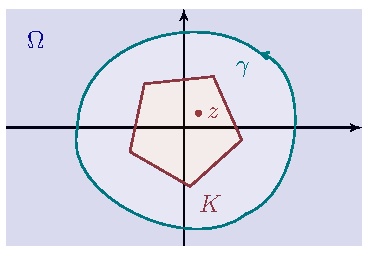
\includegraphics{Figuras/y para Gn'-Fn'.pdf}
       \end{figure}
       %
       Por hipótese, $F_n(z) \neq 0$ para todos $n\in\N$ e $z\in\Omega$, de modo
       que $F(z)\neq 0$ para todo $z\in\Omega$. Já que $F$ é holomorfa e, 
       consequentemente, contínua, podemos dizer que
       %
       \begin{equation*}
           \inf_{z\in K} |F(z)| = F(z_*) > 0.
       \end{equation*}
       %
       Portanto, podemos garantir que $G_n(z)$ é uniformemente limitada inferiormente
       em $n$ e $z\in K$. De fato,
       %
       \begin{align*}
           \inf_{z\in K} |G_n(z)| = \inf_{z\in K} |G_n(z) - F(z) + F(z)|
           \geq \inf_{z\in K} | |G_n(z) - F(z)| - |F(z)| |.
       \end{align*}
       %
       Como $G_n$ converge uniformemente para $F$, existe $n_0\in\N$ tal que
       se $n\geq n_0$, então 
       $|G_n(z) - F(z)| < \dis{\frac{1}{2} F(z_*) }$ para todo 
       $z\in K$. Logo, para todo $n\geq n_0$ temos
       %
       \begin{equation*}
           \inf_{z\in K} |G_n(z)| > \frac{1}{2}\inf_{z\in K} |F(z)| 
                                  = \frac{1}{2} F(z_*) > 0.
       \end{equation*}
       %
       Por outro lado, se $n\leq n_0$, então como $F_j(z)\neq 0$ para todo 
       $z\in\Omega$, temos que
       %
       \begin{align*}
           \inf_{z\in K} |G_n(z)| &= \inf_{z\in K} |F_1(z)|\cdots|F_n(z)| \\
                                  &\geq \prod_{j=1}^n \inf_{z\in K} |F_j(z)| \\
                                  &= |F_1(z^1_*)| \cdots |F_n(z^n_*)| \equiv I_K.
       \end{align*}
       %
       Portanto, 
       %
       \begin{equation*}
           \inf_{n\in\N} \inf_{z\in K} |G_n(z)| 
           \geq \min\left\{ I_K, \frac{1}{2}|F(z_*)| \right\} > 0,
       \end{equation*}
       %
       donde segue que 
       %
       \begin{equation*}
           \frac{G_n'}{G_n} \xrightarrow[\text{unif. em } K]{n\to\infty} \frac{F'}{F}
       \end{equation*}
       %
       para cada $z\in K$ e, como $K$ é compacto arbitrário, segue que
       %
       \begin{equation*}
           \frac{G_n'(z)}{G_n(z)} \xrightarrow{n\to\infty} \frac{F'(z)}{F(z)}
       \end{equation*}
       %
       para cada $z\in\Omega$. Observe que não podemos garantir que essa última
       convergência é uniforme em $\Omega$.
       
       Ademais, para cada $n\in\N$ temos
       %
       \begin{align*}
           \frac{G_n'(z)}{G_n(z)} 
           &= \frac{ \frac{d}{dz}[F_1(z)\cdots F_n(z)] }{F_1(z)\cdots F_n(z)} \\
           &= \sum_{j=1}^n F'_j(z)
           \frac{F_1(z)\cdots F_{j-1}(z)F_{j+1}(z)\cdots F_n(z)}{F_1(z)\cdots F_n(z)} 
           \\
           &= \sum_{j=1}^n \frac{F'_j(z)}{F_j(z)},
       \end{align*}
       %
       o que mostra que
       %
       \begin{equation*}
           \frac{F'(z)}{F(z)} = \lim_{n\to\infty} \frac{G'_n(z)}{G_n(z)}
                              = \lim_{n\to\infty} \sum_{j=1}^n \frac{F'_j(z)}{F_j(z)}
                              \equiv \sum_{j=1}^{\infty} \frac{F'_j(z)}{F_j(z)}.
       \end{equation*}
       %
    \end{proof}
    %
    
    Vamos usar este teorema para trabalhar com um exemplo interessante.
    \begin{exemplo}[A fórmula do produto da função seno]
    \index{Fórmula! do produto da função seno}
        Vamos estabelecer a validade da seguinte fórmula:
        %
        \begin{equation*}
            \frac{\sen(\pi z)}{\pi} = z\prod_{n=1}^{\infty} 
            \left( 1 - \frac{z^2}{n} \right).
        \end{equation*}
        %
        Para tanto, vamos estabelecer uma fórmula para $\cot(\pi z)$.
        Apesar de parecer estranha, a escolha da função cotangente é tudo menos
        coincidência. De fato, devido à Proposição \ref{prop:prod-inf-func-holom},
        para encontrar uma fórmula do produto da função $\sen(\pi z)/\pi$ precisaremos 
        considerar a sua derivada logarítmica, que nada mais é que $\pi\cot(\pi z)$.
        
        Vamos então mostrar que, para todo $z\in\C\setminus\mathbb{Z}$, temos
        %
        \begin{equation*}
            \pi\cot(\pi z) = \sum_{n=-\infty}^{\infty} \frac{1}{z+n}
                           \equiv \lim_{n\to\infty} \sum_{|j|\leq n} \frac{1}{z+j}
                           = \frac{1}{z} + \sum_{n=1}^{\infty} \frac{2z}{z^2 - n^2},
        \end{equation*}
        %
        onde usamos que
        %
        \begin{equation*}
            \frac{1}{z+n} + \frac{1}{z-n} = \frac{2z}{z^2 - n^2}.
        \end{equation*}
        %
        A estratégia para mostrar essa identidade será mostrar que tanto
        $F(z) = \pi\cot(\pi z)$ e $S(z) = \dis{\frac{1}{z} + 
        \sum_{n=1}^{\infty} \frac{2z}{z^2- n^2}}$ satisfazem as seguintes propriedades:
        %
        \begin{enumerate}[(i)]
            \item $H(z+1) = H(z)$;
            \item $H(z) = \dis{ \frac{1}{z} + H_0(z) }$, sendo $H_0$ analítica próxima
            do zero;
            \item $H(z)$ tem polos simples em $\Z$ e nenhuma outra singularidade.
        \end{enumerate}
        %
        De fato, para $F$,
        %
        \begin{enumerate}[(i)]
            \item 
            %
            \begin{align*}
                F(z+1)=\pi\cot(\pi(z+1)) &= \pi\frac{\cos(\pi(z+1))}{\sen(\pi(z+1))} \\
                                         &= \pi\frac{-\cos(\pi z)}{-\sen(\pi z)} \\
                                         &= \pi\cot(\pi z) \\
                                         &= F(z).
            \end{align*}
            %
            \item 
            %
            \begin{align*}
                \lim_{z\to 0} zF(z) &= \lim_{z\to 0} \pi z 
                \frac{\cos(\pi z)}{\sen(\pi z)} \\
                &= \lim_{z\to 0} \cos(\pi z)\cdot\frac{\pi z}{\sen(\pi z)} \\
                &= \lim_{z\to 0} \frac{\pi z}{\sen(\pi z)} \\
                &= 1 = \res(F,0).
            \end{align*}
            %
            Como $F$ tem apenas singularidades isoladas em $\Z$, segue do
            teorema de Laurent que para todo $z\in A(0,0,1)$ temos
            %
            \begin{equation*}
                F(z) = \frac{\res(F,0)}{z} + H_0(z) = \frac{1}{z} + H_0(z),
            \end{equation*}
            %
            com $H_0$ holomorfa em $D(0,1).$
            
            \item $F$ é claramente holomorfa em $\C\setminus\Z$.
        \end{enumerate}
        %
        Agora, para $S$, temos
        %
        \begin{enumerate}[(i)]
            \item $\forall z\in\C\setminus\Z$:
            %
            \begin{align*}
                S(z+1) &= \lim_{n\to\infty} \sum_{|j|\leq n} \frac{1}{z+1+j} \\
                       &= \lim_{n\to\infty}\left( \sum_{|j|\leq n+1} \frac{1}{z+j}
                       - \frac{1}{z-n-1} - \frac{1}{z-n} \right) \\
                       &= \lim_{n\to\infty} \sum_{|j|\leq n} \frac{1}{z_j} \\
                       &= S(z)
            \end{align*}
            %
            \item $\forall z\in D(0,1/2)$, temos
            %
            \begin{equation*}
                S(z) = \frac{1}{z} + \sum_{n=1}^{\infty} \frac{2z}{z^2 - n^2}.
            \end{equation*}
            %
            Considere a sequência de funções $h_n:D(0,1/2)\to\C$ dada por
            $h_n(z) = \dis{ \frac{2z}{z^2 - n^2} }$. Para cada $n\in\N$, temos
            que $h_n$ é uma função holomorfa e, além disso,
            %
            \begin{align*}
                \sup_{z\in D(0,1/2)} |h_n(z)| 
                = \sup_{z\in D(0,1/2)} \left| \frac{2z}{n^2
                \left( \frac{z^2}{n^2} - 1 \right)} \right|
                = \frac{2}{n^2}\sup_{z\in D(0,1/2)} 
                \frac{|z|}{\left| \frac{z^2}{n^2} - 1 \right|}
                = \frac{2}{n^2}.
            \end{align*}
            %
            Logo,
            %
            \begin{equation*}
                \sum_{n=1}^{\infty} \sup_{z\in D(0,1/2)} |h_n(z)|
                \leq 2\sum_{n=1}^{\infty} \frac{1}{n^2} < +\infty.
            \end{equation*}
            %
            Pelo teste M de Weierstrass, segue que 
            $\dis{ \sum_{n=1}^{\infty} h_n(z) \equiv S_0(z) }$ define uma função
            $S_0: D(0,1/2) \to\C$ holomorfa. Assim, 
            %
            \begin{equation*}
                S(z) = \frac{1}{z} + S_0(z),
            \end{equation*}
            %
            com $S_0$ holomorfa em $D(0,1/2)$.
            
            \item Fixado $n\in\Z$, temos que
            %
            \begin{align*}
                S(z) &= \frac{1}{z} + \sum_{j\in\N\setminus\{n\}} \frac{2z}{z^2 - j^2}
                + \frac{2z}{z^2 - n^2} \\
                &= S_1(z) + \frac{1}{z+n} + \frac{1}{z-n}.
            \end{align*}
            %
            Pelo teste M de Weierstrass, segue que $S_1(z) + \dis{\frac{1}{z+n}}$
            é holomorfa em $D(n, 1/2)$, de modo que $S$ tem apenas polos simples
            em cada ponto de $\Z$.
        \end{enumerate}
        %
        Sabendo que $F$ e $S$ satisfazem (i), (ii) e (iii), podemos afirmar que
        $H:\C\setminus\Z\to\C$ dada por
        %
        \begin{equation*}
            H(z) \equiv F(z) - S(z)
        \end{equation*}
        %
        satisfaz $H(z+1) = H(z)$. Ademais, segue da propriedade (ii) que
        $\res(H,0) = 0$, de modo que $z=0$ é uma singularidade removível de $H$.
        Esta informação, junto com a periodicidade de $H$ dada pelo item (i)
        implica que, para todo $n\in\Z$,
        %
        \begin{equation*}
            \lim_{z\to n} H(z) = \lim_{z\to n} H(z-n) = \lim_{z\to 0} H(z) = 0.
        \end{equation*}
        %
        Logo, segue do teorema de Riemann que $H$ admite extensão inteira.
        
        Para estabelecer a fórmula da cotangente, é suficiente mostrar que
        $H$ é limitada e usar o teorema de Liouville.
        
        Ademais, para mostrar que $H$ é limitada, basta trabalhar na faixa
        %
        \begin{equation*}
            S_{\frac{1}{2}} = \left\{ z\in\C : |\Re(z)| \leq \frac{1}{2} \right\},
        \end{equation*}
        %
        uma vez que $H$ satisfaz a periodicidade (i).
        %
        \begin{figure}[H]\centering
            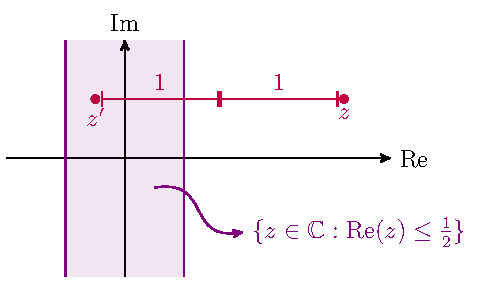
\includegraphics{Figuras/S_meio.pdf}
        \end{figure}
        %
        Já que $H:\C\to\C$ é inteira, então $H$ é limitada em
        %
        \begin{equation*}
            \Omega_1 = S_1 \cap S_{\frac{1}{2}},
        \end{equation*}
        %
        com
        %
        \begin{equation*}
            S_1 = \{ z\in\C : |\Im(z)| \leq 1 \},
        \end{equation*}
        %
        ou seja, 
        %
        \begin{equation}
            \sup_{z\in \Omega_1} |H(z)| = k_1 < +\infty
        \end{equation}
        %
        pois $\Omega_1$ é um compacto, como ilustrado abaixo.
        %
        \begin{figure}[H]\centering
            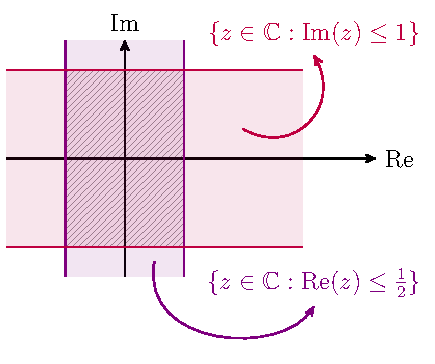
\includegraphics{Figuras/S_meio cap S_1.pdf}
            \caption{%
                A região hachurada, $\Omega_1$, é um compacto.
            }
        \end{figure}
        %
        Para terminar a demonstração que $H$ é limitada em $S_{\frac{1}{2}}$,
        resta analisar o que acontece com a função em
        %
        \begin{equation*}
            \Omega_2 = S_{\frac{1}{2}} \cap \left\{ z\in\C : |\Im(z)| > 1 \right\}.
        \end{equation*}
        %
        Ora, se $z = x+iy$, então
        %
        \begin{align*}
            \cot(\pi z) &= 
            i\frac{ e^{i\pi z} + e^{-i\pi z} }{ e^{i\pi z} - e^{-i\pi z} } \\
            &= i\frac{ e^{i\pi x}e^{-\pi y} + e^{-i\pi x}e^{\pi y} }
            { e^{i\pi x}e^{-\pi y} - e^{-i\pi x}e^{\pi y} } \\
            &= i\frac{ e^{-2\pi y} + e^{-2\pi ix} }{ e^{-2\pi y} - e^{-2\pi ix} }.
        \end{align*}
        %
        Como estamos supondo $|y|>1$, segue que
        %
        \begin{align*}
            |\cot(\pi z)| = 
            \left| 
            \frac{ e^{-2\pi y} + e^{-2\pi ix} }{ e^{-2\pi y} - e^{-2\pi ix} } 
            \right|
            \leq \frac{ 1 + e^{-2\pi y} }{ 1 - e^{-2\pi y} }
            \leq \widetilde{k_1}.
        \end{align*}
        %
        Ainda para $|y|>1$ e $|x|\leq 1/2$, temos
        %
        \begin{align*}
            \left| 
            \frac{1}{z} + \sum_{n=1}^{\infty} \frac{2z}{z^2 - n^2} 
            \right|
            &= \left| 
            \frac{1}{x+iy} + \sum_{n=1}^{\infty} \frac{2(x+iy)}{x^2 - y^2 - n^2 +2ixy} 
            \right| \\
            &\leq \frac{1}{\sqrt{x^2 + y^2}} 
            + \sum_{n=1}^{\infty} \frac{|2x|}{\sqrt{(x^2 - y^2 - n^2)^2 + 4x^2y^2}} \\
            &+ \sum_{n=1}^{\infty} \frac{|2y|}{\sqrt{(x^2 - y^2 - n^2)^2 + 4x^2y^2}} \\
            &\leq 1 
            + \sum_{n=1}^{\infty} \frac{1}{|y|^2 + n^2 - 1/4}
            + \sum_{n=1}^{\infty} \frac{|2y|}{|y|^2 + n^2 - 1/4} \\
            &\leq 1 + \sum_{n=1}^{\infty} \frac{1}{n^2} 
            + 2\sum_{n=1}^{\infty} \frac{|y|}{|y|^2/4 + n^2 - n^2/4} \\
            &\leq 1 + \frac{\pi^2}{6} + 
            8\sum_{n=1}^{\infty} \frac{|y|}{\frac{1}{4}(|y|^2 + 3n^2)} \\
            &\leq 1 + \frac{\pi^2}{6} +
            8\sum_{n=1}^{\infty} \frac{|y|}{|y|^2 + n^2}.
        \end{align*}
        %
        Agora, como $b:(0, +\infty)\to\R$ dada por $\dis{ b(x) = \frac{|y|}{|y|^2 + x^2} }$
        é decrescente já que
        %
        \begin{equation*}
            b'(x) = |y|\frac{-2x}{(|y|^2 + x^2)^2} < 0 \, \forall x+iy \in\Omega_2,
        \end{equation*}
        %
        podemos assegurar que
        %
        \begin{equation*}
            \sum_{n=1}^{\infty} \frac{|y|}{|y|^2 + n^2} 
            \leq
            \int_0^{\infty} \frac{|y|}{|y|^2 + x^2} \, dx.
        \end{equation*}
        %
        \begin{figure}[H]\centering
            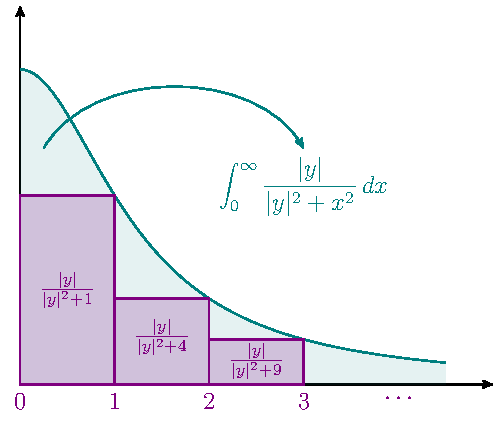
\includegraphics{%
                Figuras/majoração por integral.pdf
            }
        \end{figure}
        %
        Agora, considerando a mudança de variáveis $u = x/|y|$, temos
        %
        \begin{align*}
            \int_0^{\infty} \frac{|y|}{|y|^2 + x^2} \, dx = 
            \int_0^{\infty} \frac{1}{1 + u^2} \, du =
            \frac{\pi}{2}.
        \end{align*}
        %
        Até o momento, mostramos que
        %
        \begin{enumerate}
            \item $|\cot(\pi z)| = \dis{ 
            \left|\frac{ e^{-2\pi y} + e^{-2i\pi x} }{ e^{-2\pi y} - e^{-2i\pi x} } \right|
            \leq \frac{ 1 + e^{-2\pi y} }{ 1 - e^{-2\pi y} }
            \leq \widetilde{k_1}}$;
            
            \item $|S(z)| = \dis{ 
            \left| \frac{1}{z} + \sum_{n=1}^{\infty} \frac{2z}{z^2 - n^2} \right| 
            \leq 1 + \frac{\pi^2}{6} + 8\int_0^{\infty} \frac{|y|}{|y|^2 + x^2} \, dx
            = 1 + \frac{\pi^2}{6} + 4\pi =
            \widetilde{k_2}}$,
        \end{enumerate}
        %
        donde segue que
        %
        \begin{align*}
            \sup_{z\in\Omega_2} |H(z)| \leq 
            \sup_{z\in\Omega_2} |F(z) - S(z)| \leq
            \pi\widetilde{k_1} + \widetilde{k_2} \equiv
            k.
        \end{align*}
        %
        Portanto, lembrando que $H$ é periódica, temos
        %
        \begin{equation*}
            \sup_{z\in\C} |H(z)| =
            \sup_{z\in\Omega_1\cup\Omega_2} |H(z)| \leq
            k,
        \end{equation*}
        %
        ou seja, $H$ é limitada em $\C$.
        Pelo teorema de Liouville, como $H$ é inteira, temos
        $H(z)$ constante. 
        Agora, note que $H$ pode ser vista como extensão holomorfa de $F(z) - S(z)$,
        que é uma função ímpar. Portanto, $H$ 
        também é ímpar e $H(0) = 0$, donde segue 
        que $H\equiv 0$, ou seja, $F(z) \equiv S(z)$ e temos
        %
        \begin{equation*}
            \pi\cot(\pi z) = \frac{1}{z} + \sum_{n=1}^{\infty} \frac{2z}{z^2 - n^2},
            \, \forall z\in\C\setminus\Z.
        \end{equation*}
        %
        Finalmente, para mostrar a fórmula de produto para o seno, sejam
        %
        \begin{align*}
            G(z) &= \frac{\sen(\pi z)}{\pi} , \\
            P(z) &= z\prod_{n=1}^{\infty} \left( 1 - \frac{z^2}{n^2} \right).
        \end{align*}
        %
        Para mostrar a convergência de $P(z)$, vamos usar a 
        Proposição \ref{prop:prod-inf-func-holom} com $P(z) = zF(z)$, 
        $\Omega = D(0,R)\setminus\Z$,
        $F_n(z) = 1 - \dis{ \frac{z^2}{n^2} }$. Daí, temos
        %
        \begin{equation*}
            |F_n(z) - 1| \leq \sup_{z\in\Omega} \frac{|z|^2}{n^2} = \frac{R^2}{n^2}
            \equiv c_n.
        \end{equation*}
        %
        Portanto, para todo $z\in\Omega$,
        %
        \begin{align*}
            \frac{P'(z)}{P(z)} =
            \frac{1}{z} + \sum_{n=1}^{\infty} \frac{ -\frac{2z}{n^2} }{ 1 - \frac{z^2}{n^2} }
            = \frac{1}{z} + \sum_{n=1}^{\infty} \frac{2z}{z^2 - n^2}.
        \end{align*}
        %
        Agora, como $G'(z)/G(z) = \pi\cot(\pi z)$, 
        o resultado que acabamos de mostrar
        nos dá, para todo $z\in\Omega$,
        %
        \begin{equation*}
            \left( \frac{P(z)}{G(z)} \right)'
            = \frac{ P'(z)G(z) - P(z)G'(z) }{ G^2(z) }
            = \frac{P(z)}{G(z)}\left[ \frac{P'(z)}{P(z)} - \frac{G'(z)}{G(z)} \right]
            \equiv 0,
        \end{equation*}
        %
        de modo que $P(z) = cG(z)$ para alguma constante $c, \, \forall z\in\Omega$,
        pois $\Omega$ é conexo. 
        Ora, então
        %
        \begin{equation*}
            1 
            = \lim_{z\to 0} \prod_{n=1}^{\infty} \left( 1 - \frac{z^2}{n^2} \right)
            = \lim_{z\to 0} \frac{P(z)}{z} 
            = c\lim_{z\to 0} \frac{G(z)}{z}
            = c\lim_{z\to 0} \frac{\sen(\pi z)}{\pi z}
            = c,
        \end{equation*}
        %
        onde usamos que o produtório é holomorfo.
        Portanto, $P(z) = G(z)$ para todo $z\in\Omega$. 
        Pelo Princípio da Identidade,
        como $\Omega$ é aberto e conexo, segue que essa identidade vale para todo
        $z\in\C$.
    \end{exemplo}
    %
    \begin{exercicio}
        Use a série de Taylor de $\sin z$ e a identidade 
        % 
        \[
          \sin \pi z = \pi z\prod_{n=1}^\infty \left(1 - \frac{z^2}{n^2}\right),
        \]
        %
        deduzida acima, para demonstrar que 
        %
        \[
          \sum_{n=1}^\infty \frac{1}{n^2} = \frac{\pi^2}{6}.
        \]
    \end{exercicio}
    %
    
\section{O Teorema de Weierstrass}
    
    Anteriormente, vimos que, para construir uma função com zeros prescritos 
    na forma de uma lista ou sequência $\{a_n\}$, 
    uma tentativa ingênua era escrever
    %
    $$ f(z) = \lim_{n \to \infty} (z-a_1) \cdots (z-a_n).$$
    %
    Produtos como esse (em geral) não convergem para qualquer sequência 
    escolhida $\{a_n\}$, então essa não é a melhor escolha para construir $f$. 
    
    Mostramos, também, que vale a igualdade 
    %
    $$\frac{\sin{\pi z}}{\pi} = z \prod_{n = 1}^{\infty} \left(1 - \frac{z^2}{n^2}\right)$$
    %
    e a função $\sin{\pi z}$ se anula exatamente em $\mathbb{Z}$. 
    Analisando o produto com mais cuidado, vemos que cada fator é da forma 
    $(n^2 - z^2)/n^2 = (n - z)(n + z)/n^2$ 
    que se anula exatamente em $\pm n \in \Z$. 
    Além disso, o fato de termos escolhido fatores 
    %
    $$\left(1 - \frac{z^2}{n^2}\right)$$
    %
    em vez de $(n^2 - z^2)$ 
    nos permitiu usar a Proposição \ref{prop:prod-inf-func-holom}. 
    
    Se queremos definir uma função que se anula precisamente em uma sequência 
    qualquer $\{a_n\}$ de uma forma análoga à vista acima, ter $z^2$ nos 
    fatores pode não ser vantajoso, pois $-a_n$ pode não estar na sequência e mesmo 
    assim anular a função se $a_n$ anulá-la. Ademais, o fator $z^2$ não teve nenhuma 
    importância particular em termos de estimativas a nosso favor. Portanto, um bom 
    caminho é considerar fatores da forma
    %
    $$ \left(1 - \frac{z}{a_n}\right)g_n(z), $$
    %
    onde $g_n(z)$ são funções que facilitariam a convergência. O grande problema 
    está em como escolher tais funções e é neste ponto que reside a maior 
    contribuição de Weierstrass: ele encontrou funções que garantem a 
    convergência dada qualquer sequência $\{a_n\}$.
    
    Vamos enunciar o grande resultado desta seção agora 
    e demonstrá-lo no decorrer do texto.
    
    \begin{teorema}[Teorema do Produto de Weierstrass]
    \label{teo-Weierstrass-fatoracao}
    \index{Teorema!do Produto de Weierstrass}
        Dada uma sequência $\{a_n\}$ de números complexos tal que 
        $|a_n| \to \infty$, quando $n \to \infty$, 
        existe uma função inteira $f: \C \to \C$ que 
        se anula em $z=a_n$, para cada $n\in\mathbb{N}$, 
        e não se anula em quaisquer outros pontos do plano complexo.
        
        Além do mais, se $a_m\neq a_n$ 
        para todo $m\neq n$, então, para 
        cada $n\in\N$ temos que $z=a_n$ 
        é um zero simples de $f$ (multiplicidade um). 
    \end{teorema}
 
 \bigskip 
    
    Note que não é possível existir uma função como no enunciado do Teorema
    de Weierstrass, quando a sequência $\{a_n\}$ 
    assume infinitos valores distintos e
    a condição $|a_n| \xrightarrow{n\to\infty} \infty$ não é satisfeita.
    De fato, suponha por absurdo que exista tal função. 
    Já que $\{a_n\}$ toma infinitos valores distintos e 
    a sequência $|a_n|$ não tende a infinto, quando $n\to \infty$,
    podemos encontrar algum $R>0$ e infinitos elementos distintos 
    da sequência $\{a_n\}$ dentro do disco fechado $\overline{D(0,R)}$. 
    Desta forma, segue da compacidade de $\overline{D(0,R)}$, 
    que existe alguma 
    subsequência $\{a_{n_{k}}\}$ de $\{a_n\}$, formada também
    por elementos distintos, que converge
    para algum ponto $w\in \overline{D(0,R)}$.
    Isto é, $a_{n_{k}}\to w$, quando $k\to\infty$.
    Como $f(a_{n_{k}})=0$, para  todo $k\in\mathbb{N}$ 
    e $f$ é contínua, então segue que 
    $f(w)=f(\lim_{k\to\infty} a_{n_k})=\lim_{k\to\infty} f(a_{n_k}) =0$.  
    Logo $w$ é um zero de $f$ que é um ponto aderente à uma 
    sequência de zeros de $f$. Portanto segue do Princípio da Identidade 
    que $f\equiv 0$. Mas isto é um absurdo, pois estamos assumindo 
    que $a_1, a_2, \dots$ são os únicos zeros de $f$.
 
 
 \bigskip 
 
    
    Vamos introduzir agora um dos ingredientes mais importantes da prova
    do Teorema de Weierstrass, que são os chamados fatores canônicos. 
    Para cada $k \in \N$, definimos 
    o fator canônico de grau $k$ por
    \index{Fatores Canônicos}
    %
    \[
    E_k(z) = (1-z)\exp{\left(z + \frac{z^2}{2} + \cdots + \frac{z^k}{k}\right)}.
    \]
    %
    Para $k=0$, definimos $E_0(z) = 1-z$ Observe que a 
    função $E_k(z/w)$ se anula apenas em $z = w$ (se $w \neq 0$). 
    %
    \begin{lema}
    \label{lema-wstr-est-factor}
    Se $|z| \leq 1/2$, então, para algum $c>0$, 
    temos $|1-E_k(z)| \leq c|z|^{k+1}$ qualquer 
    que seja $k$ inteiro não negativo.
    \end{lema}
    %
    \begin{proof}
    Podemos escolher um ramo do logaritmo adequado 
    de modo que vale a equação $1-z = \exp{\log(1-z)}$. 
    Além disso, da série geométrica, sabemos que 
    %
    \[
    \frac{1}{1-z} = \sum_{n=0}^{\infty}z^n 
    \]
    %
    já que $|z| \leq 1/2 < 1$. Integrando esta equação, obtemos que
    %
    \[ 
    \log(1-z) = - \sum_{n=0}^{\infty}\frac{z^n}{n}.
    \]
    %
    Observe que 
    %
    \begin{align*}
        E_k(z) &= \exp{\left(\log(1-z) + z + \cdots + \frac{z^k}{k}\right)} \\
        &= \exp\left(-\sum_{n=k+1}^{\infty}\frac{z^n}{n}\right) \\
        &= \exp{w}.
    \end{align*}
    %
    Agora, estimamos $|w|$:
    %
    \begin{align*}
        |w| &= \left | -\sum_{n=k+1}^{\infty}\frac{z^n}{n} \right | \\
        &\leq |z|^{k+1}\sum_{n=k+1}^{\infty}\frac{|z|^{n - (k+1)}}{n} \\
        &\leq |z|^{k+1}\sum_{n=0}^{\infty}|z|^n \\
        &\leq |z|^{k+1}\sum_{n=0}^{\infty} 2^{-n} \\
        &= 2|z|^{k+1} \leq 2 \frac{1}{2^{k+1}} \leq 1.
    \end{align*}
    %
    Portanto,
    %
    \begin{align*}
        |1 - E_k(z)| = |1 - \exp{w}| 
        &= \left | \sum_{n=1}^{\infty}\frac{w^n}{n!} \right | \\
        &\leq |w|\sum_{n=1}^{\infty}\frac{|w|^{n-1}}{n\cdot (n-1)!} \\
        &\leq |w|\sum_{n=0}^{\infty}\frac{|w|^n}{n!} \\
        &\leq |w|\sum_{n=0}^{\infty}\frac{1}{n!} \\
        &=|w|e \leq 2e|z|^{k+1}.
    \end{align*}
    %
    Tomando $c = 2e$, temos o resultado.
    \end{proof}
    %
    
    Observe que, neste lema, a escolha $|z| \leq 1/2$ é 
    feita por motivos de simplicidade. Em termos práticos 
    poderíamos escolher $|z| \leq \alpha$ para $\alpha \in (0,1)$.
    
    Dada uma função inteira $f$, se $a$ é um zero de ordem 
    $m$ de $f$, então existe uma função inteira $g$ tal que
    %
    \[ 
    f(z) = (z-a)^mg(z) 
    \]
    %
    e $g(a) \neq 0$. Portanto, para os nossos propósitos, 
    podemos supor que a sequência de zeros no Teorema de 
    Weierstrass não contém o zero. Vamos mostrar que função 
    %
    \[ 
    f(z) = z^m \prod_{n=1}^{\infty}E_n(z/a_n)
    \]
    %
    tem um zero de ordem $m$ na  origem e se anula em $a_n$ 
    para todo $n$ e em nenhum outro ponto.
    
    Seja $R>1$ e denote $D_R = D(0,R)$. Existe $n_0 \in \N$ tal que 
    %
    \begin{align*}
        \begin{cases}
            |a_n| < 2R, \text{ se } n \leq n_0 \\
            |a_n| \geq 2R, \text{ se } n > n_0
        \end{cases},
    \end{align*}
    %
    pois supomos que $|a_n| \to \infty$. Note que a função 
    %
    \[
    z^m\prod_{n=1}^{n_0}E_n(z/a_n)
    \]
    %
    é inteira e se anula precisamente em $z = 0$ e $z = a_n$ com 
    $n \leq n_0$. Para $n > n_0$, temos $|a_n| \geq 2R$ e segue que
    %
    \[
    \left | \frac{z}{a_n} \right | \leq \frac{|z|}{2R} < \frac{R}{2R} = \frac{1}{2}
    \]
    %
    sempre que $|z| < R$. Do Lema \ref{lema-wstr-est-factor} 
    concluímos que 
    $|1 - E_n(z/a_n)| \leq c|z/a_n|^{n+1} \leq c2^{-(n+1)}$ 
    para $z \in D_R$ e $n > n_0$. 
    Pela Proposição \ref{prop:prod-inf-func-holom}, concluímos que 
    %
    \[
    \prod_{n=n_0 + 1}^{\infty}E_n(z/a_n)
    \]
    %
    converge uniformemente em $D_R$ para uma função holomorfa 
    e que não se anula em $D_R$.
    
    Para cada $R$, concluímos que a função 
    %
    \[
    f_R (z) = z^m\left(\prod_{n=1}^{n_0}E_n(z/a_n)\right)\left(\prod_{n=n_0 + 1}^{\infty}E_n(z/a_n)\right)
    \]
    %
    é holomorfa em $D_R$ e se anula precisamente em $z = 0$ 
    e nos pontos da sequência $\{a_n\}$ no interior de $D_R$. 
    Podemos reescrever a expressão acima numa forma mais conveniente:
    %
    \begin{align*}
        f_R (z) &= z^m \cdot \prod_{n=1}^{n_0}E_n(z/a_n) \cdot \lim_{N \to \infty}\prod_{n=n_0 + 1}^{N}E_n(z/a_n) \\
        &= \lim_{N \to \infty} \left( z^m \cdot \prod_{n=1}^{n_0}E_n(z/a_n) \right) \cdot \prod_{n=n_0 + 1}^{N}E_n(z/a_n) \\
        &= \lim_{N \to \infty}  z^m \cdot \prod_{n=1}^{N}E_n(z/a_n) \\
        &= z^m \prod_{n=1}^{\infty}E_n(z/a_n).
    \end{align*}
    %
    Por construção, é simples ver que, se $R'>R$, então 
    $f_{R'}|_{D_R} = f_R$, ou seja, $f_{R'}$ 
    é uma extensão analítica de $f_R$. Isto mostra que a aplicação
    %
    \[
    z \mapsto z^m \prod_{n=1}^{\infty}E_n(z/a_n)
    \]
    %
    está bem definida para todo $z \in \C$, pois $R$ é arbitrário 
    e define uma função que satisfaz as conclusões do Teorema de Weierstrass.
    
    A força deste teorema pode ser vista por uma consideração simples. 
    Como saber se um produtório da forma
    %
    $$\prod_{n=1}^{\infty} \left( 1 - \frac{z}{a_n} \right)$$
    %
    converge? Pela Proposição \ref{prop:prod-inf-func-holom}, 
    um caminho seria analisar se a soma 
    %
    \[
    \sum_{n=1}^{\infty} \left | \frac{z}{a_n} \right |
    \]
    %
    converge ou não. Isto naturalmente impõe condições sobre a sequência em questão. 
    Utilizando o que foi construído no Teorema de Weierstrass, 
    podemos considerar sequências arbitrárias. Uma consequência disso é que, 
    além dos zeros, podemos escolher suas multiplicidades, 
    já que um mesmo valor pode se repetir na sequência.
    %
    \begin{corolario}
    Se duas funções $f_1$ e $f_2$ satisfazem as 
    condições do Teorema de Weierstrass, então $f_1(z) = f_2(z)\exp{g(z)}$ 
    para alguma função inteira $g(z)$. 
    \end{corolario}
    %
    \begin{observacao}
        O corolário acima é essencialmente a solução ao seguinte problema:
        dada $f_2$ inteira, como obter $f_1$ 
        inteira e com os mesmos zeros de $f_2$?
        Um raciocínio heurístico que nos ajuda a 
        esclarecer a resposta é o seguinte:
        atendendo à preservação dos zeros, 
        é claro que não se pode fazer sobre $f_2$ 
        operações como translação e inversão, e intuitivamente 
        ficamos mesmo só com operações de rotação e 
        expansão (ou contração), que podem ser executadas 
        simultaneamente pela exponencial complexa.
        Finalmente, $f_1$ ser inteira pede que o 
        argumento da exponencial também seja inteiro, 
        e portanto $f_1=f_2 \exp g(z)$ para alguma $g$ inteira.
    \end{observacao}
    %
    \begin{proof}
    Seja $h(z) = f_1(z)/f_2(z)$. Se $f_1$ e $f_2$ 
    ambas se anulam em um ponto $a$, 
    então este é um zero de mesma multiplicidade para ambas, 
    ou seja, $f_i(z) = (z-a)^mg_i(z)$ com $g_i$ holomorfa e 
    $g_i(a) \neq 0$ para  $i = 1,2$ e $m$ natural. 
    
    Tomando o limite de $h(z)$ quando $z \to a$, 
    vemos que o limite existe e é não nulo, logo, 
    $a$ é uma singularidade removível de $h$, então podemos estender $h$ 
    para todo o plano complexo fazendo 
    $h(a) = \lim_{z \to a} h(z)$ para cada singularidade $a$.
    
    Usando a mesma notação para $h$ e sua extensão, temos que ela é inteira. 
    Como $\C$ é simplesmente conexo, 
    segue do Lema \ref{lema-ramo-log} que $h(z) = \exp{g(z)}$ 
    para alguma função $g$ inteira.
    \end{proof}
    %
    
    \subsection{Interpolações e o Teorema de Weierstrass}
    
    
    Nesta seção vamos apresentar uma aplicação muito 
    interessante do Teorema de Weierstrass. 
    Ela é baseada também em outro importante teorema, 
    conhecido como Teorema de Mittag-Leffler 
    (veja abaixo, Teorema \ref{teo-mittag-leffler}). 
    
    
    Um dos problemas mais clássicos de 
    interpolação polinomial consiste em: 
    fornecido um conjunto finito de pares 
    de números complexos (ou reais) da forma
    %
    \[
    (z_1,w_1), (z_2,w_2), \ldots, (z_n,w_n);
    \]
    %
    encontrar um polinômio $P$ de menor grau possível 
    cujo gráfico contém todos estes pares de pontos, 
    ou seja, $P(z_j)=w_j$ para cada $j=1,\ldots,n$. 
    Às vezes, nos referimos a um polinômio 
    satisfazendo esta propriedade como um 
    polinômio interpolador e os pares de
    números complexos $(z_i,w_i)$, com $i=1,\ldots,n$ como dados.
    
    Caso o conjunto de dados acima não possua nenhuma propriedade especial, em geral, um 
    polinômio interpolador para estes dados 
    terá grau no mínimo $n-1$. 
    Na verdade, Lagrange mostrou
    que este problema sempre 
    admite uma solução com um polinômio de grau exatamente $n-1$. 
    Tais polinômios são chamados, hoje em dia, 
    de polinômios interpoladores de Lagrange
    \index{polinômios interpoladores}. 
    Para o conjunto de dados fornecidos acima, 
    o polinômio interpolador de Lagrange tem a forma 
    %
    \[
    P(z)
    =
    \sum_{j=1}^n 
    w_j  
    \frac
    {(z-z_1)(z-z_2)\cdots (z-z_{j-1})(z-z_{j+1})\cdots (z-z_n)}
    {(z_j-z_1)(z_j-z_2)\cdots (z_j-z_{j-1})(z_j-z_{j+1})\cdots (z_j-z_n)}
    \]
    %
    
    No que segue, usamos os Teoremas 
    de Weierstrass e Mittag-Leffler para mostrar que dada
    uma sequência infinita de números complexos 
    distintos $(z_n)_{n\in\N}$ e uma sequência arbitrária
    $(w_n)_{n\in\N}$, se $|z_n|\xrightarrow{n\to\infty}\infty$, 
    então podemos construir uma
    função inteira $f:\C\to\C$ tal que 
    $f(z_n)=w_n$, para todo $n\in\mathbb{N}$.
    Note que esta aplicação pode ser vista 
    como um resultado de interpolação e que, na verdade, 
    generaliza o esquema de interpolação baseado nos 
    polinômios de Lagrange, mas
    para o caso de uma interpolação 
    em que a função deve se ajustar a um 
    conjunto infinito enumerável de valores. 
    
    
    
    \bigskip 
    
    Como mencionado acima, para resolver o problema 
    de interpolação, por uma função inteira, 
    de um conjunto infinito de dados, vamos
    precisar do Teorema de Mittag-Leffler. Este é um resultado
    de natureza análoga à do Teorema de Weierstrass, 
    mas que ao invés de considerar o problema de zeros prescritos,
    considera o problema de existência de uma 
    função meromorfa
    em $\C$ cujas singularidades são 
    polos de ordem e localização prescritos por 
    alguma sequência de números complexos 
    $(z_n)$ satisfazendo $|z_n|\xrightarrow{n\to\infty}\infty$.
    
    
    \begin{teorema}[Teorema de Mittag-Leffler]
    \label{teo-mittag-leffler}
    \index{Teorema!de Mittag-Leffler}
    Seja $(z_n)_{n\in\mathbb{N}}$ uma 
    sequência de número complexos distintos com 
    $|z_n|\xrightarrow{n\to\infty}\infty$. 
    Seja $(P_n)_{n\in\N}$ uma sequência qualquer de polinômios 
    não-nulos tais que $P_n(0)=0$, 
    para todo $n\in\N$. 
    Então existe uma função $f$ meromorfa em 
    $\C$ cujas singularidades são apenas os pontos da sequência $(z_n)_{n\in\N}$ e a parte
    principal da série de Laurent de $f$ em torno de
    $z_n$ é dada exatamente por $P_n\big(1/(z-z_n)\big)$,
    isto é, para cada $n\in\N$, 
    existe um raio positivo $r_n$ dado por
    $r_n \equiv \inf\{|z_n-z_j|: j\in \N\setminus\{n\} \}$ 
    tal que para todo ponto $z$ 
    do anel aberto $A(z_n,0,r_n)$ temos
    %
    \[
    f(z) = P_n\left(\frac{1}{z-z_n}\right)+h_n(z),
    \]
    %
    onde $h_n:D(z_n,r_n)\to\C$ é uma função holomorfa.
    \end{teorema}
    
    
    A maneira mais natural de pensar em como este teorema 
    poderia ser provado  seria
    considerando a seguinte série de funções: 
    \[
     f(z) = \sum_{n=1}^{\infty} P_n\left( \frac{1}{z-z_n}  \right).
    \]
    Entretanto, como o leitor já deve estar imaginando, 
    esta tentativa esbarraria no problema
    da convergência desta série, 
    já que no enunciado do teorema é permitido escolher 
    a sequência  $(z_n)_{n\in\N}$ de forma muito geral. 
    Não obstante, veremos que a prova é baseada nesta ideia:
    ao invés de considerarmos exatamente esta série, 
    vamos construir uma outra série de funções que 
    é basicamente uma modificação da série acima, onde 
    cada parcela desta nova série é obtida
    subtraindo-se uma função holomorfa apropriada 
    de cada uma das parcelas da série acima. 
    
    
    
    
    \begin{proof}[Prova do Teorema de Mittag-Leffer]
    Primeiro vamos assumir que $z_n\neq 0$, para todo $n\in\N$.
    Desta forma 
    $U\equiv \C\setminus\{z_1,z_2,\ldots\}$ 
    é um domínio contendo a origem do plano complexo.
    
    
    Para cada $n\in\N$, temos que a função $g_n:U\to\mathbb{C}$
    dada por
    %
    \[
    g_n(z) = P_n\left(\frac{1}{z-z_n}\right),
    \]
    %
    define uma função analítica em $U$. 
    Observe que a única singularidade de 
    $g_n$ é o ponto $z=z_n$. 
    Portanto, podemos garantir para todo $z\in D(0,|z_n|)$ que
    %
    \[
    g_n(z) = \sum_{k=0}^{\infty} \frac{g_{n}^{(k)}(0)}{k!}z^k. 
    \]
    %
    Além do mais, para cada $n\in\N$, existe $k_n\in\mathbb{N}$ tal que
    %
    \begin{equation}
    \label{eq-aux1-teo-mittag-leffer}
    \left| 
    g_n(z) - \sum_{k=0}^{k_n} \frac{g_{n}^{(k)}(0)}{k!}z^k
    \right|
    =
    \left| 
    \sum_{k=k_n+1}^{\infty} \frac{g_{n}^{(k)}(0)}{k!}z^k
    \right|
    \leq 
    \frac{1}{2^n},\quad \forall z\in \overline{D(0,|z_n|/2)}.
    \end{equation}    
    %
    Para cada $n\in\N$, considere a função $f_n:U\to\C$ dada por
    %
    \[
    f_n(z) = P_n\left(\frac{1}{z-z_n}\right)- \sum_{k=0}^{k_n} \frac{g_{n}^{(k)}(0)}{k!}z^k.
    \]
    %
    Claramente $f_n$ é uma função holomorfa em $U$. 
    
    O próximo passo é mostrar que a função $f$ dada
    pela seguinte série de funções 
    %
    \[
    f\equiv \sum_{n=1}^{\infty} f_n,
    \]
    %
    está bem definida em $U$ e, além disso, define uma
    função holomorfa neste domínio. 
    Para provar estas afirmações a ideia é 
    usar o Teste M de Weierstrass. 
    
    Seja $K\subset U$ um subconjunto compacto arbitrário. 
    Como $|z_n|\xrightarrow{n\to\infty}\infty$, podemos 
    garantir que existe algum 
    $n_0\in\N$ tal que $K\subset \overline{D(0,|z_n|/2)}$ 
    para todo $n\geqslant n_0$. 
    
    Usando a desigualdade \eqref{eq-aux1-teo-mittag-leffer}
    e as observações acima, podemos garantir que
    %
    \[
    \sum_{n=n_0}^{\infty} \sup_{z\in K}|f_n(z)|
    \leqslant 
    \sum_{n=n_0}^{\infty} \sup_{z\in \overline{D(0,|z_n|/2)}} |f_n(z)|
    \leqslant 
    \sum_{n=n_0}^{\infty} \frac{1}{2^n}
    \leqslant
    2.
    \]
    %
    Logo, segue da continuidade das $f_j$'s em $K$ 
    e da desigualdade acima que
    %
    \[
    \sum_{n=1}^{\infty} \sup_{z\in K} |f_n(z)|
    \leqslant
    \sum_{n=1}^{n_0} \sup_{z\in K} |f_n(z)|
    +2
    <+\infty.
    \]
    %
    Como $K$ é um subconjunto arbitrário de $U$, segue do teste
    M de Weierstrass que a série de funções 
    $\sum_{n=1}^{\infty}f_n$ define uma função holomorfa em $U$,
    que denotaremos por $f$. 
    
    Para finalizar a prova do Teorema,
    precisamos obter a série de Laurent de $f$ 
    em torno de cada uma de suas singularidades.
    
    Para cada $n\in\mathbb{N}$, seja 
    $r_n \equiv \inf\{ |z_n-z_j|: j\in\N\setminus\{n\}\}$. 
    Considere a função $q_n:A(z_n,0,r_n)\to\C$ dada por
    %
    \[
    q_n(z) = f(z)-f_n(z) \equiv 
    f(z)- P_n\left(\frac{1}{z-z_n}\right) +
    \sum_{k=0}^{k_n} \frac{g_{n}^{(k)}(0)}{k!}z^k.
    \]
    %
    Para finalizar a prova, basta mostrar 
    que $z_n$ é a única singularidade
    da função $q_n$ em $D(z_n,r_n)$ 
    e que esta singularidade 
    é removível, pois já
    que $P_j(0)=0$, para todo $j\in\N$,
    podemos obter, imediatamente, da identidade abaixo
    %
    \[
    f(z) = P_n\left(\frac{1}{z-z_n}\right) + q_n(z)+
    \sum_{k=0}^{k_n} \frac{g_{n}^{(k)}(0)}{k!}z^k
    \]
    %
    que $P_n(1/(z-z_n))$ é a parte principal da 
    série de Laurent de $f$ no anel $A(z_n,0,r_n)$.
    
    
    Para mostrar a validade da afirmação feita acima, 
    note que pela definição de $f$ e $f_n$, temos para todo
    $z\in A(z_n,0,r_n)$ que
    %
    \begin{align*}
    q_n(z) 
    &= 
    f(z)- P_n\left(\frac{1}{z-z_n}\right) +
    \sum_{k=0}^{k_n} \frac{g_{n}^{(k)}(0)}{k!}z^k  
    \\[0.4cm]
    &=
    \sum_{k=1}^{\infty} f_k(z)
    - P_n\left(\frac{1}{z-z_n}\right) +
    \sum_{k=0}^{k_n} \frac{g_{n}^{(k)}(0)}{k!}z^k
    \\[0.4cm]
    &=
    \sum_{k=1}^{\infty} f_k(z) - f_n(z)
    \\[0.4cm]
    &=
    \sum_{k\in \N\setminus\{n\}} f_k(z).
    \end{align*}
    %
    Para finalizar a prova só precisamos mostrar que o 
    limite abaixo existe
    %
    \begin{equation}
    \label{eq-aux2-teo-mittag-leffer}
    \lim_{z\to z_n} q_n(z) 
    = 
    \lim_{z\to z_n} \sum_{k\in \N\setminus\{n\}} f_k(z)
    = 
    \sum_{k\in \N\setminus\{n\}} \lim_{z\to z_n} f_k(z)
    =
    \sum_{k\in \N\setminus\{n\}} f_k(z_n).
    \end{equation}    
    %
    Para mostrar que a afirmação acima é verdadeira,
    vamos apelar mais uma vez para o Teste M de Weierstrass.
    Primeiro, observe que para todo $k\in\N$ com $k\neq n$, temos
    da definição de $r_n$ que a função 
    $f_k$ é holomorfa em $D(z_n,r_n)$, 
    para cada $k\in\N\setminus\{n\}$. 
    Usando novamente que $|z_n|\xrightarrow{n\to\infty}\infty$,
    podemos afirmar que existe algum $n_1\in\N$
    tal que $n_1\geqslant n$  e além do mais, 
    para todo $k\geqslant n_1$, 
    temos que $D(z_n,r_n)\subset \overline{D(0,|z_k|/2)}$.
    Seja $K$ um subconjunto compacto arbitrário do disco aberto $D(z_n,r_n)$. 
    Então segue da estimativa 
    \eqref{eq-aux1-teo-mittag-leffer} e da continuidade de $f_k$ em
    $D(z_n,r_n)$ que 
    %
    \begin{align*}
    \sum_{k\in \N\setminus\{n\}} \sup_{z\in K}|f_k(z)|
    &=
    \sum_{k=1}^{n-1}\sup_{z\in K}|f_k(z)|
    +
    \sum_{k=n+1}^{n_1}\sup_{z\in K}|f_k(z)|
    +
    \sum_{n=n_1+1}^{\infty}\sup_{z\in K}|f_k(z)|
    \\[0.4cm]
    &\leqslant
    \sum_{k=1}^{n-1}\sup_{z\in K}|f_k(z)|
    +
    \sum_{k=n+1}^{n_1}\sup_{z\in K}|f_k(z)|
    +
    \sum_{k=n_1+1}^{\infty}\sup_{z\in \overline{D(0,|z_k|/2)}}|f_k(z)|
    \\[0.4cm]
    &\leqslant
   \sum_{k=1}^{n-1}\sup_{z\in K}|f_k(z)|
    +
    \sum_{k=n+1}^{n_1}\sup_{z\in K}|f_k(z)|
    +    
    \sum_{k=n_1+1}^{\infty}\frac{1}{2^k}
    <+\infty.
    \end{align*}
    %
    Já que $K\subset D(z_n,r_n)$ é um compacto abritário, segue da 
    estimativa acima e do teste M de Weierstrass
    que a série de funções
    %
    \[
    \sum_{k\in \N\setminus\{n\}} f_k
    \]
    %
    define uma função holomorfa em $D(z_n,r_n)$.
    Em particular, esta série de funções é uma função contínua 
    em $D(z_n,r_n)$ e, portanto, existe o 
    limite em \eqref{eq-aux2-teo-mittag-leffer}
    e isto encerra a prova do teorema para o caso em que
    todos os termos da sequência $(z_n)_{n\in\N}$
    são não-nulos. 
    
    
    \medskip 
    
    Para o caso em que um elemento da sequência $(z_n)_{n\in\N}$ 
    se anula, digamos $z_1=0$,
    consideramos a sequência $z_2,z_3,\ldots$ e 
    construímos as funções $f_2,f_3,\ldots$ como
    no caso anterior. Em seguida, definimos para 
    cada $z\in\C\setminus \{0,z_2,\ldots\}$
    \[
    f(z) = P_1\left(\frac{1}{z}\right) +\sum_{n=2}^{\infty}f_n(z).
    \]
    Então podemos argumentar como no caso anterior 
    e mostrar que todas as singularidades de $f$ ocorrem
    nos pontos $\{z_1=0,z_2,z_3,\ldots\}$ e que a série de Laurent de $f$ é determinada como no enunciado do teorema. 
    Esta última observação finalmente encerra a prova do Teorema de Mittag-Leffler.
    \end{proof}
    
    
    
    
    
    \begin{teorema}[Teorema de Interpolação]
    Dada uma sequência de números complexos distintos
    $(z_n)_{n\in\N}$ e uma sequência arbitrária $(w_n)_{n\in\N}$, 
    se $|z_n|\xrightarrow{n\to\infty}\infty$
    então é possível 
    encontrar uma função inteira $f:\C\to\C$ tal 
    que $f(z_n)=w_n$, para todo $n\in\N$.
    \end{teorema}
    
    
    \begin{proof}
    Já que $(z_n)_{n\in\N}$ é uma sequência de números
    complexos distintos segue, do Teorema do Produto de 
    Weiertrass que existe uma função inteira $g:\C\to\C$
    tal que $z=z_n$ é um zero simples de $g$, para cada $n\in\N$. 
    Além do mais, a função $g$ não se anula em nenhum
    outro ponto do plano complexo. 
    Da analiticidade de $g$ segue que, para cada $n\in\N$, existe uma função 
    inteira $g_n$ que não se anula no 
    disco aberto $D(z_n,r_n)$, para algum $r_n>0$,
    e satisfaz 
    %
    \[
    g(z) = (z-z_n)g_n(z), \quad\forall z\in\C.
    \]
    %
    Já que $g_n(z_n)\neq 0$, podemos observar que está bem definido, 
    para cada $n\in\N$, o seguinte polinômio de grau um  
    %
    \[
    P_n(z) = \frac{w_n}{g_n(z_n)}\cdot z.
    \]
    %
    Como para todo $n\in\N$ temos $P_n(0)=0$, 
    podemos aplicar o 
    Teorema de Mittag-Leffler para garantir a existência 
    de uma função $h$, meromorfa em $\C$,
    cujas singularidades são dadas pelos pontos da
    sequência $(z_n)_{n\in\N}$ e tal que a série de Laurent 
    de $h$ em torno $z=z_n$ é dada por 
    %
    \[
    h(z) 
    = 
    P_n\left( \frac{1}{z-z_n}\right)+h_n(z)
    =
    \frac{w_n}{g_n(z_n)}\cdot \frac{1}{z-z_n} +h_n(z),
    \]
    %
    para todo $z\in A(z_n,0,\rho_n)$, para algum $\rho_n>0$
    e para alguma função holomorfa $h_n:D(z_n,\rho_n)\to\C$.
    
    Como, para cada $n\in\N$ temos que $z=z_n$ é um zero 
    simples de $g$ e também um polo simples de $h$, segue que
    $z=z_n$ é uma singularidade removível da função 
    $f:\C\setminus\{z_1,z_2,\ldots\}\to\C$ dada por
    $f(z)=g(z)h(z)$. 
    
    Para finalizar a prova do teorema basta observar
    que temos, para cada $n\in\N$,
    %
    \begin{align*}
    f(z_n)
    =
    \lim_{z\to z_n}f(z)
    &=
    \lim_{z\to z_n}
    g(z)h(z)
    \\
    &=
    \lim_{z\to z_n}
    (z-z_n)g_n(z)
    \left( \frac{w_n}{g_n(z_n)} \cdot\frac{1}{z-z_n}+h_n(z) \right)
    \\
    &=
    \lim_{z\to z_n}
    \left( 
    w_n\frac{g_n(z)}{g_n(z_n)}
    +
    (z-z_n)g_n(z)h_n(z) 
    \right)
    =
    w_n.
    \end{align*}
    %
    \end{proof}
    %
    
    \section{O Teorema da Fatoração de Hadamard}
    Nesta seção vamos discutir um refinamento do teorema da fatoração de Weierstrass,
    enunciado como teorema de Hadamard. Esse teorema combina os resultados que discutimos
    sobre o crescimento de uma função e sua quantidade de zeros com o teorema de
    Weierstrass. Recorde que o teorema de Weierstrass afirma que uma função inteira
    que se anula em $0, a_1, a_2, \dots$ e em nenhum outro ponto tem a forma
    %
    \[
        e^{g(z)}z^m\prod_{n=1}^{\infty} E_n(z/a_n),
    \]
    %
    para alguma função $g$ inteira.
    Hadamard refinou este resultando mostrando que, no caso de funções de ordem finita,
    o grau dos fatores canônicos pode ser tomado constante e $g$ é um polinômio.
    
    A título de lembrete, dizemos que uma função inteira tem ordem de crescimento no máximo
    $\rho > 0$ se $|f(z)| \leq A\exp(B|z|^{\rho}), \, \forall z\in\C$. A ordem de 
    crescimento de $f$ é, então, o ínfimo de todos os $\rho$ que satisfazem essa
    condição. Recorde também que mostramos que se $f$ tem ordem de crescimento no
    máximo $\rho$ então
    %
    \[
        n_f(r) \leq Cr^{\rho}, \quad r \gg 1,
    \]
    %
    onde $n_f(r)$ denota os zeros de $f$ em $D(0, r)$. Antes de seguir para o teorema, 
    recorde por último que se $a_1, a_2, \dots \in\C^*$ são zeros de $f$ e $\rho < s$
    então
    %
    \[
        \sum_{n=1}^{\infty} \frac{1}{|a_n|^s} < +\infty.
    \]
    %
    Vamos ao enunciado do teorema.
    %
    \begin{teorema}[Teorema da Fatoração de Hadamard]
    \index{Teorema!da Fatoração de Hadamard}
    \label{teo:fatoracao-hadamard}
        Suponha que $f:\C\to\C$ é uma função inteira com ordem de crescimento $\rho_0$.
        Seja $k\equiv \lfloor \rho_0 \rfloor \in \Z$. 
        Se $a_1, a_2, \ldots \in\C^*$ são os 
        zeros não-nulos de $f$, então
        %
        \[
            f(z) = \exp(P(z))z^m\prod_{n=1}^{\infty} E_k(z/a_n),
        \]
        %
        onde $P$ é um polinômio de grau menor ou igual a $k$ e $m$ é a multiplicidade
        de $z=0$ como zero de $f$.
    \end{teorema}
    %
    Vamos precisar de alguns lemas auxiliares para demonstrar esse resultado.
    %
    \begin{lema}
    \label{lema:majoracao}
        $x+1 > x^\alpha, \, \forall x>0$, 
        $0 < \alpha < 1$.
    \end{lema}
    %
    Este lema nos será muito útil em algumas majorações, e o usaremos sem cerimônia.
    %
    \begin{proof}
        Para $x>0$ e $0<\alpha<1$,
        $x \mapsto (x+1)^{1/\alpha}$ 
        é estritamente crescente. 
        Como $x + 1 > 1$ e $1/\alpha > 1$ ,
        $(x+1)^{1/\alpha} > (x+1) > x$,
        e, portanto, 
        $(x+1)^{1/\alpha} > x$, 
        o que implica em
        $x+1 > x^\alpha$. 
    \end{proof}
    %
    \begin{lema}
    \label{lema:5.2-Stein}
        Os produtos canônicos satisfazem as seguintes desigualdades:
        %
        \begin{enumerate}[i)]
            \item $\exp( -2|z|^{k+1} ) \leq |E_k(z)|, \, |z| \leq 1/2$;
            \item $|1 - z|\exp( -c(k)|z|^k ) \leq |E_k(z)|, \, |z| \geq 1/2$,
        \end{enumerate}
        %
        sendo $c(k)$ uma constante positiva e finita que depende de $k$.
    \end{lema}
    %
    \begin{proof}
        \begin{enumerate}
            \item[{\it i)}] Para $z\in\C$ tal que $|z| \leq 1/2$, temos que 
            $1-z\in\C\setminus L_{\pi}$ e podemos escrever
            %
            \[
                \log(1-z) = -\sum_{n=0}^{\infty} \frac{z^n}{n},
            \]
            %
            onde $\log$ denota o ramo principal do logaritmo. Logo,
            %
            \begin{align*}
                E_k(z) = \exp\left( \log(1-z) + \sum_{n=1}^k \frac{z^n}{n} \right)
                       = \exp\left( -\sum_{n=k+1}^{\infty} \frac{z^n}{n} \right)
                       \equiv \exp(w).
            \end{align*}
            %
            Já que $\exp(-w) \leq |\exp(w)|$ e $|w| \leq 2|z|^{k+1}$ (demonstração
            do Lema \ref{lema-wstr-est-factor}), temos que
            %
            \[
                \exp(-2|z|^{k+1}) \leq \exp(-|w|) \leq |\exp(w)| = |E_k(z)|,
            \]
            %
            e está verificada a validade de {\it i)}.
            
            \item[{\it ii)}] Por definição, para todo $k\geq 1$ temos que
            %
            \begin{align*}
                |E_k(z)| &= |1-z| \cdot \left| 
                \exp \left( z + z^2/2 + \cdots + z^k/k \right) 
                \right| \\[0.3cm]
                &\geq |1 - z| \cdot \exp 
                \left( -\left| z + z^2/2 + \cdots + z^k/k \right| \right),
            \end{align*}
            %
            onde usamos que $|e^z| \geq e^{-|z|}$. Agora, se $|z| \geq 1/2$ então
            segue da desigualdade triangular que
            %
            \begin{align*}
                -\left| z + z^2/2 + \cdots + z^k/k \right| 
                &\geq -|z| - |z^2|/2 - \cdots - |z^k|/k \\[0.3cm]
                &= -|z|^k\left( 
                \frac{1}{|z|^{k-1}} + \frac{1}{2|z|^{k-2}} + \cdots + \frac{1}{k} \right) \\[0.3cm]
                &\geq -|z|^k\left( 2^{k-1} + \frac{2^{k-2}}{2} + \cdots + \frac{1}{k} \right)\\[0.3cm]
                &\equiv -|z|^k c(k).
            \end{align*}
            %
            Logo, para $|z| \geq 1/2$ temos
            %
            \[
                |1 - z|\exp(-c(k)|z|^k) \leq |E_k(z)|,
            \]
            %
            encerrando a prova do item {\it ii)} e do lema.
        \end{enumerate}
    \end{proof}
    %
    
    A prova do teorema de Hadamard se baseia em cotas inferiores para o produto
    dos fatores canônicos quando $z$ está longe das raízes $a_1, a_2, \dots$.
    Nesse teorema, o ``grau'' dos produtos canônicos é constante e igual a $k$
    e não varia como no teorema de Weierstrass. Por isso, vamos trabalhar para obter
    essas estimativas para os casos em que $z$ está no complemento de pequenos discos
    centrados nas raízes citadas acima.
    %
    \begin{lema}
    \label{lema:5.3-Stein}
        Sejam $k = \lfloor \rho_0 \rfloor$ e $s>0$ tal que $\rho_0 < s < k+1$.
        Então existe uma constante $C \equiv C(k,s)$, que depende de $k$ e $s$,
        tal que
        %
        \[
            \exp\left( -C(k,s) |z|^s \right) \leq \left| 
                                             \prod_{n=1}^{\infty} E_k(z/a_n) 
                                             \right|,
        \]
        %
        para todo $z\in\C\setminus\dis\bigcup_{n=1}^{\infty} 
        D\left( a_n, \frac{1}{|a_n|^{k+1}} \right)$.
    \end{lema}
    %
    \begin{proof}
        A prova deste lema é delicada. Recorde que como os $a_n$ são
        zeros de $f$, temos que $|a_n| \xrightarrow{n\to\infty} +\infty$,
        de modo que podemos supor, sem perda de generalidade, que $|a_n| \geq 1$.
        Para começar, vamos mostrar que o produtório de $E_k(z/a_n)$ converge.
        
        Pelo Lema \ref{lema-wstr-est-factor}, existe $n_0\in\N$ tal que se $n\geq n_0$
        então
        %
        \begin{equation*}
            \left| E_k(z/a_n) - 1 \right| 
            \leq 2e\left| \frac{z}{a_n} \right|^{k+1}
            = 2e|z|^{k+1}\cdot\frac{1}{|a_n|^{k+1}}.
        \end{equation*}
        %
        Uma vez que $1 \leq |a_n|$ e $\rho_0 < s < k+1$, temos 
        $|a_n|^s \leq |a_n|^{k+1}$. Utilizando essa desigualdade na estimativa acima,
        segue que
        %
        \begin{equation*}
            \left| E_k(z/a_n) - 1 \right|
            \leq 2e|z|^{k+1}\cdot\frac{1}{|a_n|^{k+1}}
            \leq 2e|z|^{k+1}\cdot\frac{1}{|a_n|^s}.
        \end{equation*}
        %
        Portanto,
        %
        \begin{equation*}
            \sum_{n=n_0}^{\infty} \left| E_k(z/a_n) - 1 \right|
            \leq 2e|z|^{k+1} \sum_{n=n_0}^{\infty} \frac{1}{|a_n|^s} < +\infty
        \end{equation*}
        %
        e obtemos
        %
        \begin{equation*}
            \Big |\prod_{n=1}^{\infty} E_k(z/a_n) \Big | < \infty.
        \end{equation*}
        %
        Logo, podemos reescrever o produtório como
        %
        \begin{equation*}
            \prod_{n=1}^{\infty} E_k(z/a_n)
            = \prod_{\substack{n\in\N \\ |a_n| \leq 2|z|}}^{\infty} E_k(z/a_n) \cdot 
            \prod_{\substack{n\in\N \\ |a_n| > 2|z|}}^{\infty} E_k(z/a_n).
        \end{equation*}
        %
        Observe que o primeiro dos produtos no lado direito tem uma quantidade finita
        de fatores, enquanto que o segundo tem uma quantidade infinita. Vamos obter
        cotas inferiores semelhantes à do enunciado do lema para cada um deles,
        começando pelo segundo.
        
        Temos, usando o fato de que $|z/a_n| < 1/2$ e o Lema \ref{lema:5.2-Stein},
        que
        %
        \begin{align*}
            \left|
            \prod_{\substack{n\in\N \\ |a_n| > 2|z|}}^{\infty} E_k(z/a_n)
            \right|
            =
            \prod_{\substack{n\in\N \\ |a_n| > 2|z|}}^{\infty} \left|E_k(z/a_n)\right|
            \geq
            \prod_{\substack{n\in\N \\ |a_n| > 2|z|}}^{\infty} \exp\left( 
            -2\left| \frac{z}{a_n} \right|^{n+1}
            \right).
        \end{align*}
        %
        Agora, o último produtório pode ser reescrito como
        %
        \begin{equation*}
            \prod_{\substack{n\in\N \\ |a_n| > 2|z|}}^{\infty} \exp\left( 
            -2\left| \frac{z}{a_n} \right|^{n+1}
            \right)
            =
            \exp\left( 
            -2|z|^{k+1} \sum_{\substack{n\in\N \\ |a_n| > 2|z|}} \frac{1}{|a_n|^{k+1}}
            \right).
        \end{equation*}
        %
        Agora, vamos estimar o somatório. Note que, como $|a_n| > 2|z|$, temos
        %
        \begin{equation*}
            \frac{1}{|a_n|^{k+1}} 
            = \frac{1}{|a_n|^s|a_n|^{k+1-s}}
            \leq \frac{1}{|a_n|^s 2^{k+1-s}|z|^{k+1-s}}.
        \end{equation*}
        %
        Daí,
        %
        \begin{equation*}
            \sum_{\substack{n\in\N \\ |a_n| > 2z}} \frac{1}{|a_n|^{k+1}}
            \leq
            \frac{1}{2^{k+1-s}|z|^{k+1-s}}
            \sum_{\substack{n\in\N \\ |a_n| > 2|z|}} \frac{1}{|a_n|^s} 
            < +\infty,
        \end{equation*}
        %
        de maneira que
        %
        \begin{align*}
            \left|
            \prod_{\substack{n\in\N \\ |a_n| > 2|z|}}^{\infty} E_k(z/a_n)
            \right|
            &\geq 
            \exp\left(
            -2|z|^{k+1} \cdot \frac{1}{2^{k+1-s}|z|^{k+1-s}}
            \sum_{\substack{n\in\N \\ |a_n| > 2|z|}} \frac{1}{|a_n|^s}
            \right) \\
            &\equiv 
            \exp\left(
            -C_1(k,s) |z|^s
            \right),
        \end{align*}
        %
        sendo
        %
        \begin{equation*}
            C_1(k,s) = 2^{s-k}
            \sum_{\substack{n\in\N \\ |a_n| > 2|z|}} \frac{1}{|a_n|^s}.
        \end{equation*}
        %
        Agora, para obter cotas inferiores para o primeiro produto, a saber
        %
        \begin{equation*}
            \prod_{\substack{n\in\N \\ |a_n| \leq 2|z|}}^{\infty} E_k(z/a_n),
        \end{equation*}
        %
        usamos o item ii) do Lema \ref{lema:5.2-Stein} para escrever
        %
        \begin{equation*}
            \left|
            \prod_{\substack{n\in\N \\ |a_n| \leq 2|z|}} E_k(z/a_n)
            \right| \geq
            \prod_{\substack{n\in\N \\ |a_n| \leq 2|z|}} \left| 1 - \frac{z}{a_n} \right|
            \prod_{\substack{n\in\N \\ |a_n| \leq 2|z|}} \exp\left( -c(k)|z/a_n|^k \right),
        \end{equation*}
        %
        sendo $c(k)$ como na demonstração do item ii) do Lema \ref{lema:5.2-Stein}.
        Agora, note que
        %
        \begin{equation*}
            \prod_{\substack{n\in\N \\ |a_n| \leq 2|z|}} \exp\left( -c(k)|z/a_n|^k \right)
            =
            \exp\left( 
            -c(k)|z|^k \sum_{\substack{n\in\N \\ |a_n| \leq 2|z|}} \frac{1}{|a_n|^k}
            \right).
        \end{equation*}
        %
        Daí, como $s-k > 0$ por hipótese, temos
        %
        \begin{equation*}
            |a_n|^{-k} = |a_n|^{-s}|a_n|^{s-k} \leq |a_n|^{-s} 2^{s-k} |z|^{s-k}.
        \end{equation*}
        %
        Assim, obtemos a seguinte cota inferior
        %
        \begin{align*}
            \exp
            \left( 
            -c(k)|z|^k \sum_{\substack{n\in\N \\ |a_n| \leq 2|z|}} \frac{1}{|a_n|^k}
            \right)
            &\geq
            \exp
            \left( 
            -c(k)|z|^k|z|^{s-k}2^{s-k} \sum_{\substack{n\in\N \\ |a_n| \leq 2|z|}} \frac{1}{|a_n|^s}
            \right) \\
            &=
            \exp
            \left( 
            -C_2(k,s)|z|^s
            \right),
        \end{align*}
        %
        sendo
        %
        \begin{equation*}
            C_2(k, s) = -c(k) 2^{s-k} \sum_{\substack{n\in\N \\ |a_n| \leq 2|z|}} \frac{1}{|a_n|^s}.
        \end{equation*}
        %
        Agora, para estimar
        %
        \begin{equation*}
            \prod_{\substack{n\in\N \\ |a_n| \leq 2|z|}} \left| 1 - \frac{z}{a_n} \right|,
        \end{equation*}
        %
        vamos usar o fato de que $z$ está longe dos discos de centro $a_n$ e raio $1/|a_n|^{k+1}$,
        ou seja, que $|a_n - z| \geq 1/|a_n|^{k+1}$ para todo $n\in\N$. Daí, segue que
        %
        \begin{align*}
            \prod_{\substack{n\in\N \\ |a_n| \leq 2|z|}} \left| 1 - \frac{z}{a_n} \right|
            &=
            \prod_{\substack{n\in\N \\ |a_n| \leq 2|z|}} \left| \frac{a_n - z}{a_n} \right| \\
            &\geq
            \prod_{\substack{n\in\N \\ |a_n| \leq 2|z|}} \frac{1}{|a_n|^{k+1}}\cdot\frac{1}{|a_n|} \\
            &=
            \prod_{\substack{n\in\N \\ |a_n| \leq 2|z|}} \frac{1}{|a_n|^{k+2}}.
        \end{align*}
        %
        Precisamos agora estimar o último produtório acima. Lembrando que ele
        é finito, vamos tomar o logaritmo natural 
        e utilizar a estimativa de Jensen para o número de zeros de $f$ para obter
        %
        \begin{align*}
            \ln\left( \prod_{\substack{n\in\N \\ |a_n| \leq 2|z|}} \frac{1}{|a_n|^{k+2}} \right)
            &=
            \sum_{\substack{n\in\N \\ |a_n| \leq 2|z|}} -\ln\left( |a_n|^{k+2} \right) \\[0.4cm]
            &= 
            -(k+2)\sum_{\substack{n\in\N \\ |a_n| \leq 2|z|}} \ln|a_n| \\[0.4cm]
            &\geq 
            -(k+2)\sum_{\substack{n\in\N \\ |a_n| \leq 2|z|}} \ln(2|z|) \\[0.4cm]
            &\geq 
            -(k+2) n_f(2|z|) \ln(2|z|) \\[0.4cm]
            &\geq
            -(k+2) C_3(k, s) |z|^s \ln(2|z|) \\[0.4cm]
            &\geq
            -(k+2) C_4(k, s) |z|^{s + \e}, \\[0.4cm]
            &=
            -C_5(k,s) |z|^{s + \e} \, \ \ \ \ \forall \e > 0.
        \end{align*}
        %
        Na quinta desigualdade, usamos $n_f(2|z|) \leq C|z|^{\rho_0}$ pela estimativa do número de zeros. A constante $C_3(k,s)$ é escolhida de modo que $C|z|^{\rho_0} < C_3(k,s)|z|^s$ levando em conta os casos em que $|z|< 1$ ou $|z| \geq 1$. Na sexta desigualdade, escolhemos $C_4(k,s)$ de tal forma que $\ln(2|z|) \leq C_4(k,s)|z|^\e$. Portanto, obtemos
        %
        \begin{equation*}
            \prod_{\substack{n\in\N \\ |a_n| \leq 2|z|}} \frac{1}{|a_n|^{k+2}}
            \geq
            \exp
            \left(
            -C_5(k, s) |z|^{s + \e}
            \right), \, \forall \e > 0.
        \end{equation*}
        %
        Para juntar esta estimativa com a estimativa para o produtório de $\exp(-c(k)|z/a_n|^k)$,
        primeiro observamos que
        %
        \begin{align*}
            \prod_{\substack{n\in\N \\ |a_n| \leq 2|z|}} \exp\left( -c(k)|z/a_n|^k \right)
            \geq
            \exp
            \left( 
            -C_2(k,s)|z|^s
            \right)
            \geq
            \exp
            \left( 
            -C_6(k,s)|z|^{s + \e}
            \right), \, \forall \e > 0.
        \end{align*}
        %
        Daí, temos finalmente que
        %
        \begin{equation*}
            \left|
            \prod_{\substack{n\in\N \\ |a_n| \leq 2|z|}} E_k(z/a_n)
            \right| 
            \geq
            \exp
            \left(
            -C_7(k, s) |z|^{s + \e}
            \right),
        \end{equation*}
        %
        sendo $C_7 \equiv C_5 + C_6$. Para verificar que esta desigualdade encerra
        a prova do lema, observamos que
        %
        \begin{equation*}
            \left|
            \prod_{\substack{n\in\N \\ |a_n| > 2|z|}}^{\infty} E_k(z/a_n)
            \right|
            \geq
            \exp
            \left(
            -C_1(k, s) |z|^s
            \right)
            \geq
            \exp
            \left(
            -C_8(k, s) |z|^{s + \e}
            \right), \, \forall \e > 0.
        \end{equation*}
        %
        Por fim, basta notar que o argumento inteiro vale para qualquer 
        $s \in (\rho_0, k+1)$, basta escolher $\e > 0$ tal que
        $s + \e \in (\rho_0 , k+1)$ temos
        %
        \begin{align*}
            \left|
            \prod_{n=1}^{\infty} E_k(z/a_n)
            \right|
            = 
            \left|
            \prod_{\substack{n\in\N \\ |a_n| \leq 2|z|}}^{\infty} E_k(z/a_n) 
            \right|
            \cdot
            \left|
            \prod_{\substack{n\in\N \\ |a_n| > 2|z|}}^{\infty} E_k(z/a_n)
            \right|
            \geq
            \exp
            \left(
            -C_9(k, s) |z|^{s + \e},
            \right)
        \end{align*}
        %
        sendo $C_9 \equiv C_7 + C_8$. Já que qualquer número real em $(\rho_0, k+1)$
        pode ser escrito como $s + \e$ para algum $s \in (\rho_0, k+1)$ e $\e > 0$,
        finalizamos a prova do lema.
    \end{proof}
    %
    \begin{corolario}
    \label{cor-seq-raios-inf}
        Existe uma sequência $r_1, r_2, \dots, r_m, \dots,$ com $r_m \to \infty$ tal que
        %
        \begin{equation*}
            \left|
            \prod_{n=1}^{\infty} E_k(z/a_n)
            \right|
            \geq
            \exp(-C|z|^s),
        \end{equation*}
        %
        para
        %
        \begin{equation*}
            z \in \bigcup_{n=1}^{\infty} \partial D(0, r_n).
        \end{equation*}
        %
    \end{corolario}
    %
    \begin{proof}
        Já que $\rho_0 < s < k+1$, temos
        %
        \begin{equation*}
            \sum_{n=1}^{\infty} \frac{1}{|a_n|^{k+1}} < +\infty.
        \end{equation*}
        %
        Portanto, existe $n_0\in\N$ tal que se $n\geq n_0$ então
        %
        \begin{equation*}
            \sum_{n = n_0 + 1}^{\infty} \frac{1}{|a_n|^{k+1}} < \frac{1}{10}.
        \end{equation*}
        %
        Sendo assim, dados inteiros consecutivos $L$ e $L+1 \gg 1$, podemos
        encontrar $r\in [L, L+1]$ tal que
        %
        \begin{equation*}
            \partial D(0, r) 
            \cap 
            \bigcup_{n=1}^{\infty} D\left( a_n, \frac{1}{|a_n|^{k+1}} \right)
            =
            \varnothing.
        \end{equation*}
        %
        De fato, se não existisse tal $r$ então a união dos fechados
        %
        \begin{equation*}
            I_n = 
            \left[
            |a_n| - \frac{1}{|a_n|^{k+1}}, |a_n| + \frac{1}{|a_n|^{k+1}}
            \right],
        \end{equation*}
        %
        que têm comprimento $2/|a_n|^{k+1}$, formaria uma cobertura de $[L, L+1]$
        %
        \begin{figure}[H]\centering
            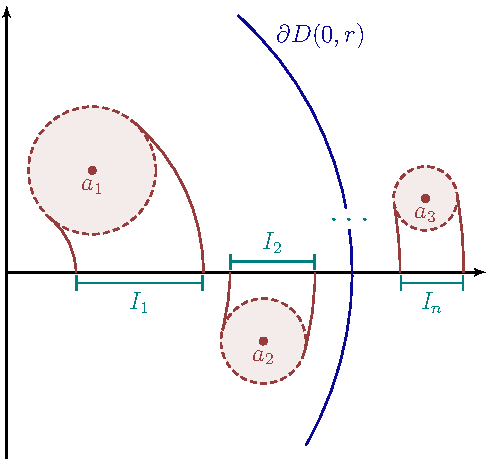
\includegraphics{%
                Figuras/In Hadamard.pdf
            }
        \end{figure}
        %
        Ora, mas a união dos $I_n$ não pode cobrir $[L, L+1]$ já que
        %
        \begin{align*}
            \Leb\left(
            \bigcup_{n=n_0}^{\infty} I_n
            \right) 
            \leq
            \sum_{n=n_0}^{\infty} \Leb(I_n)
            =
            \sum_{n=n_0}^{\infty} \frac{2}{|a_n|^{k+1}}
            <
            \frac{2}{10},
        \end{align*}
        %
        enquanto que $\Leb([L, L+1]) = 1$. Portanto, podemos encontrar 
        a sequência desejada $(r_n)_{n\in\N}$ com $r_n \xrightarrow{n\to\infty} \infty$
        aplicando o Lema \ref{lema:5.3-Stein}.
    \end{proof}
    %
    
    \medskip
    
    Antes de rumar para a demonstração do teorema de Hadamard, vamos precisar de um último
    lema.
    %
    \begin{lema}
    \label{lema:5.5-Stein}
        Suponha que $g:\C\to\C$ é inteira e tal que
        %
        \begin{equation*}
            \Re(g(z)) \leq C r^s, \, |z| = r, \, s > 0
        \end{equation*}
        %
        para uma sequência de números reais positivos $r$ que tende para o infinito.
        Então $g$ é um polinômio de grau menor ou igual a $s$.
    \end{lema}
    %
    \begin{proof}
        Expandindo $g$ em série de potências ao redor da origem, temos
        %
        \begin{equation*}
            g(z) = \sum_{n=0}^{\infty} a_n z^n.
        \end{equation*}
        %
        Usando a fórmula integral de Cauchy, temos que
        %
        \begin{equation*}
            \frac{1}{2\pi} \int_0^{2\pi} g(re^{i\theta}) e^{-in\theta} \, d\theta
            =
            \begin{cases}
                a_n r^n, n \geq 0 \\
                0, n < 0
            \end{cases}.
        \end{equation*}
        %
        Tomando conjugados complexos, obtemos
        %
        \begin{equation*}
            \frac{1}{2\pi} \int_0^{2\pi} \overline{ g(re^{i\theta}) } e^{-in\theta} \, d\theta = 0
        \end{equation*}
        %
        sempre que $n > 0$. Como $2\Re(g) = g + \overline{g}$, adicionamos as duas equações
        acima para obter
        %
        \begin{equation*}
            a_n r^n = \frac{1}{\pi} \int_0^{\pi} \Re(g(re^{i\theta}))e^{-in\theta} \, d\theta,
            \, n > 0.
        \end{equation*}
        %
        Para $n = 0$, tomamos a parte real em ambos os lados da primeira integral para encontrar
        %
        \begin{equation*}
            2\Re(a_0) = \frac{1}{\pi}\int_0^{2\pi} \Re(g(re^{i\theta})) \, d\theta.
        \end{equation*}
        %
        Agora, notamos o fato de que para todo $n\neq 0$ a integral de $e^{-in\theta}$
        em qualquer circunferência de centro na origem é nula. Portanto,
        %
        \begin{equation*}
            a_n 
            = 
            \frac{1}{\pi r^n} \int_0^{2\pi} \left[ \Re(g(re^{i\theta})) - Cr^s \right]e^{-in\theta}
            \, d\theta, \, n > 0,
        \end{equation*}
        %
        e segue que
        %
        \begin{equation*}
            |a_n| 
            \leq
            \frac{1}{\pi r^n} 
            \int_0^{2\pi} \left[ Cr^s - \Re(g(re^{i\theta})) \right] \, d\theta
            \leq
            2CR^{s-n} - 2\Re(a_0)r^{-n}.
        \end{equation*}
        %
        Fazendo $r\to\infty$, obtemos que $a_n = 0$ para $n > s$, de modo que $g$
        é um polinômio de grau no máximo $s$, como desejado.
    \end{proof}
    %
    
    \medskip
    
    Agora, para provar o teorema de Hadamard, seja
    %
    \begin{equation*}
        E(z) = z^m \prod_{n=1}^{\infty} E_k(z/a_n).
    \end{equation*}
    %
    Para mostrar que $E$ é inteira, notamos que
    %
    \begin{equation*}
        |1 - E_k(z/a_n)| \leq c\left| \frac{z}{a_n} \right|^{k+1}
    \end{equation*}
    %
    para todo $n$ suficientemente grande também que
    %
    \begin{equation*}
        \sum_{n=0}^{\infty} \frac{1}{|a_n|^{k+1}}
    \end{equation*}
    %
    converge, pois $\rho_0 < s < k+1$. Além disso, $E$ tem os mesmos zeros 
    que $f$, de modo que $f/E$ é holomorfa e não se anula em lugar nenhum,
    ou seja,
    %
    \begin{equation*}
        \frac{f(z)}{E(z)} = e^{g(z)}
    \end{equation*}
    %
    para alguma função inteira $g$. Como $f$ tem ordem de crescimento
    $\rho_0$ e pela estimativa para $E$ obtida no Corolário \ref{cor-seq-raios-inf},
    temos
    %
    \begin{align*}
        \exp(\Re(g(z))) &= \left| \frac{f(z)}{E(z)} \right| \\
                        &\leq \frac{A_1 \exp( B_1|z|^{\rho_0} )}{A_2 \exp( -B_2|z|^{s} )} \\
                        &= A_1 \exp(B_1 |z|^{\rho_0} + B_2 |z|^s) \\
                        &\leq A_1 \exp(B_3 |z|^s).
    \end{align*}
    %
    para $|z| = r_m$. Isso mostra que
    %
    \begin{equation*}
        \Re(g(z)) \leq A_2|z|^s, \, |z| = r_m
    \end{equation*}
    %
    e segue do Lema \ref{lema:5.5-Stein} que $g$ é um polinômio de grau menor
    ou igual a $s$, terminando a demonstração.
    %
    % falar do teo de Mittag-Leffler e da aplicação para funções com imagens prescritas (?)
 
 
 
 
 
    \subsection{O Pequeno Teorema de Picard}
    
    Nesta seção vamos mostrar, como consequência do Teorema de Hadamard, um resultado fascinante devido a Picard. Ele afirma, entre outras coisas, 
    que a imagem de uma função inteira, de ordem de crescimento finita, pode omitir no máximo um ponto do plano complexo! 
    Isto é, se $f:\C\to\C$ é uma função inteira com ordem de 
    crescimento $0\leqslant \rho<+\infty$, então a o conjunto imagem $f(\C)$ 
    é todo o plano complexo, exceto possivelmente um ponto.
    Este resultado é conhecido como o {\it Pequeno Teorema de Picard}. Seu enunciado mais preciso é apresentado logo abaixo.
 
    
        %
        \begin{teorema}[Pequeno Teorema de Picard]
        \label{teo:pequeno-picard}
        \index{Pequeno Teorema de Picard}
            Se $f:\C\to\C$ é uma função inteira não constante e com ordem de crescimento 
            $\rho \in [0,+\infty)$, então
            %
            \[
              \sharp (f(\C))^c \leq 1.
            \]
            %
            Além do mais,
            \begin{itemize}
                \item se $0\leqslant \rho<1$, então $f(\C)=\C$; 
                
                \item se $1\leqslant \rho<+\infty$, então 
                a imagem de $f$ omite no máximo um ponto do plano complexo 
                e todo ponto da imagem de $f$ possui infinitas pré-imagens.
            \end{itemize}
        \end{teorema}

        \medskip 
        %
        Antes de apresentar a prova do Teorema de Picard vamos enunciar um pequeno lema preliminar.
        
        \medskip 
        %
        \begin{lema}
        \label{lema-pol-sobrejetor}
            Todo polinômio não constante $P:\C\to\C$ é sobrejetor.
        \end{lema}
        %
        \begin{proof}[Demonstração do lema]
            Dado $w\in\C$, o polinômio $P(z) - w$ é não constante e, pelo
            Teorema Fundamental da Álgebra, tem uma raiz $z_w$. Ora, então
            $P(z_w) = w$ e, portanto, $P$ é sobrejetor.
        \end{proof}
        
        \medskip
        %
        Vamos, então, à demonstração do Pequeno Teorema de Picard.
        %
        \begin{proof}[Demonstração do Pequeno Teorema de Picard]
            Suponha que existe algum $a\in\C$ tal que
            %
            \[
            f(z) - a \neq 0, \quad \forall z\in\C.
            \]
            %
            Em outras palavras, estamos supondo que a função inteira $g:\C\to\C$ 
            dada por $g(z)= f(z)-a$ não possui raízes. 
            Observe que $g$ é uma função inteira de ordem de crescimento 
            finito $\rho$. Portanto, podemos aplicar o Teorema da 
            Fatoração de Hadamard (Teorema \ref{teo:fatoracao-hadamard}) 
            para garantir que 
            %
            \begin{align}
            \label{eq-aux1-litle-picard}
                f(z) - a = e^{P(z)},
            \end{align}
            %
            onde $P(z)$ é um polinômio de grau no máximo $\rho$.
            
            \medskip 
            Vamos separar o restante do argumento em dois casos.
            \begin{itemize}
                \item Caso 1. $0\leqslant \rho<1$;
                \item Caso 2. $1<\rho<+\infty$.
            \end{itemize}
            \medskip 
            
            
            Caso 1. Neste caso, como $0\leqslant \rho<1$, então  
            segue do Teorema da Fatoração de Hadamard que
            o polinômio que aparece no lado direito de
            \eqref{eq-aux1-litle-picard} é tal que
            $\textrm{grau}(P)=\lfloor \rho \rfloor =0$, ou seja, 
            $P$ é constante. Mas então existe 
            alguma constante $K\in \C$ tal que 
            $f(z)-a=e^K$ para todo $z\in\C$ o que 
            é um absurdo, pois por hipótese estamos assumindo que 
            $f$ é não-constante. 
            
            O absurdo vem de termos assumido que existe um número complexo $a$ tal que a função $g=f-a$ não possui raízes. Desta forma, para todo $a\in\C$ fixado, existe algum $z\in \C$ 
            tal que $f(z)=a$ e, portanto, $f(\C)=\C$.
            
            
            
            
            \bigskip 
            Caso 2. 
            Já que todo ponto não-nulo do plano complexo
            pode ser representado em coordenadas polares, podemos afirmar que dado um ponto arbitrário 
            $b\in \C\setminus\{a\}$,
            existe algum $\varphi \in [0, 2\pi)$ tal que
            %
            \[
            b - a = |b - a| e^{i\varphi}.
            \]
            %
            Usando o Lema \ref{lema-pol-sobrejetor},
            podemos garantir que existe um número complexo $z_b\in\C$ tal que
            %
            \begin{align*}
                P(z_b) = \ln|b-a| + i\varphi.
            \end{align*}
            %
            Substituindo $z$ por $z_b$ em
            \eqref{eq-aux1-litle-picard} e usando a igualdade acima ficamos com
            %
            \[
            f(z_b) - a = b - a \iff f(z_b) = b.
            \] 
            %
            Consequentemente, a  
            imagem do $f$ pode omitir 
            no máximo um ponto de $\C$.
            
            Para mostrar que a imagem inversa de qualquer ponto 
            $b\in \C\setminus\{a\}$ possui infinitos pontos, basta 
            observar que para cada $k\in\Z$, podemos usar 
            novamente o Lema \ref{lema-pol-sobrejetor}
            para garantir que existe um ponto 
            $z_{b,k}\in \C$
            tal que 
            \begin{align*}
                P(z_{b,k}) = \ln|b-a| + i(\varphi+2k\pi).
            \end{align*}
            Argumentando de maneira análoga, 
            concluímos que 
            $f(z_{b,k})=b$. 
            Já que para qualquer par de inteiros distintos $k$ e $k'$
            temos $z_{b,k}\neq z_{b,k'}$, pois 
            $\Im(P(z_{b,k}))\neq \Im(P(z_{b,k'}))$, 
            segue que $b$ tem infinitas pré-imagens. 
            Como $b\in \C\setminus\{a\}$
            é arbitrário, finalizamos a prova do teorema.
        \end{proof}
        %